\documentclass{article}

\usepackage{arxiv}

\usepackage[utf8]{inputenc} % allow utf-8 input
\usepackage[T1]{fontenc}    % use 8-bit T1 fonts
\usepackage{lmodern}        % https://github.com/rstudio/rticles/issues/343
\usepackage{hyperref}       % hyperlinks
\usepackage{url}            % simple URL typesetting
\usepackage{booktabs}       % professional-quality tables
\usepackage{amsfonts}       % blackboard math symbols
\usepackage{nicefrac}       % compact symbols for 1/2, etc.
\usepackage{microtype}      % microtypography
\usepackage{lipsum}
\usepackage{graphicx}

\title{Simultaneously estimating food web connectance and structure with
uncertainty}

\author{
    Anubhav Gupta
    \thanks{Corresponding author}
   \\
    Department of Evolutionary Biology and Environmental Studies \\
    University of Zurich \\
  8057 Zurich, Switzerland \\
  \texttt{\href{mailto:anubhav.gupta@ieu.uzh.ch}{\nolinkurl{anubhav.gupta@ieu.uzh.ch}}} \\
   \And
    Reinhard Furrer
   \\
    Department of Mathematics and Department of Computational Science \\
    University of Zurich \\
  8057 Zurich, Switzerland \\
  \texttt{\href{mailto:reinhard.furrer@math.uzh.ch}{\nolinkurl{reinhard.furrer@math.uzh.ch}}} \\
   \And
    Owen L. Petchey
   \\
    Department of Evolutionary Biology and Environmental Studies \\
    University of Zurich \\
  8057 Zurich, Switzerland \\
  \texttt{\href{mailto:owen.petchey@ieu.uzh.ch}{\nolinkurl{owen.petchey@ieu.uzh.ch}}} \\
  }


% Pandoc citation processing
\newlength{\csllabelwidth}
\setlength{\csllabelwidth}{3em}
\newlength{\cslhangindent}
\setlength{\cslhangindent}{1.5em}
% for Pandoc 2.8 to 2.10.1
\newenvironment{cslreferences}%
  {}%
  {\par}
% For Pandoc 2.11+
\newenvironment{CSLReferences}[3] % #1 hanging-ident, #2 entry spacing
 {% don't indent paragraphs
  \setlength{\parindent}{0pt}
  % turn on hanging indent if param 1 is 1
  \ifodd #1 \everypar{\setlength{\hangindent}{\cslhangindent}}\ignorespaces\fi
  % set entry spacing
  \ifnum #2 > 0
  \setlength{\parskip}{#2\baselineskip}
  \fi
 }%
 {}
\usepackage{calc} % for calculating minipage widths
\newcommand{\CSLBlock}[1]{#1\hfill\break}
\newcommand{\CSLLeftMargin}[1]{\parbox[t]{\csllabelwidth}{#1}}
\newcommand{\CSLRightInline}[1]{\parbox[t]{\linewidth - \csllabelwidth}{#1}}
\newcommand{\CSLIndent}[1]{\hspace{\cslhangindent}#1}

\usepackage{lineno}
\linenumbers
\usepackage {amsmath}
\setlength\parindent{24pt}
\usepackage{setspace}\doublespacing
\usepackage{booktabs}
\usepackage{longtable}
\usepackage{array}
\usepackage{multirow}
\usepackage{wrapfig}
\usepackage{float}
\usepackage{colortbl}
\usepackage{pdflscape}
\usepackage{tabu}
\usepackage{threeparttable}
\usepackage{threeparttablex}
\usepackage[normalem]{ulem}
\usepackage{makecell}


\begin{document}
\maketitle

\def\tightlist{}


\begin{abstract}
\begin{enumerate}
\def\labelenumi{\arabic{enumi})}
\tightlist
\item
  Food web models explain and predict the trophic interactions in a food
  web, and they can infer missing interactions among the organisms. The
  allometric diet breadth model (ADBM) is a food web model based on the
  foraging theory. In the ADBM the foraging parameters are
  allometrically scaled to body sizes of predators and prey. In Petchey
  et al.~(2008), the parameterisation of the ADBM had two limitations:
  (a) the model parameters were point estimates, and (b) food web
  connectance was not estimated.
\item
  The novelty of our current approach is: (a) we consider multiple
  predictions from the ADBM by parameterising it with approximate
  Bayesian computation, to estimate parameter distributions and not
  point estimates. (b) Connectance emerges from the parameterisation, by
  measuring model fit using the true skill statistic, which takes into
  account prediction of both the presences and absences of links.
\item
  We fit the ADBM using approximate Bayesian computation to 12 observed
  food webs from a wide variety of ecosystems. Connectance was
  consistently overestimated in the new parameterisation method. In some
  of the food webs, considerable variation in estimated parameter
  distributions occurred, and resulted in considerable variation
  (i.e.~uncertainty) in predicted food web structure.
\item
  These results lend weight to the possibility that the observed food
  web data is missing some trophic links that do actually occur. It also
  seems likely that the ADBM likely predicts some links that do not
  exist. The latter could be addressed by accounting in the ADBM for
  additional traits other than body size. Further work could also
  address the significance of uncertainty in parameter estimates for
  predicted food web responses to environmental change.
\end{enumerate}
\end{abstract}

\keywords{
    connectance
   \and
    ABC
   \and
    ADBM
   \and
    food web
   \and
    true skill statistic
   \and
    uncertainty
  }

\hypertarget{introduction}{%
\section{Introduction}\label{introduction}}

Knowledge about the trophic interactions among the organisms in a
community is crucial for understanding the structure and dynamics of
ecological communities and for predicting their response to
environmental change (Dunne, Williams, and Martinez 2002; Tylianakis and
Binzer 2014; O'Connor et al. 2009; Bergamino, Lercari, and Defeo 2011;
Krause et al. 2003; Lurgi, L'opez, and Montoya 2012; Morris, Sinclair,
and Burwell 2015). The network of trophic interactions is often referred
to as a food web. The food web structure can provide answers to key
ecological questions: which species are more vulnerable to environmental
changes such as temperature (Petchey et al. 1999); how robust a food web
is to extinctions (Dunne, Williams, and Martinez 2002); and how a food
web reacts if the predators are removed (Knight et al. 2005)?

Trophic interactions information from multiple sources can be used to
infer a food web, e.g.~gut contents (Peralta-Maraver, López-Rodríguez,
and de Figueroa 2016) and cannot be assigned with certainty to a
specific prey item (Baker, Buckland, and Sheaves 2014). With stable
isotope ratios of tissues, uncertainty may be due to factors such as
variability in the isotopic fractionation values across multiple
combinations of diets and tissues/species, unquantified temporal or
spatial variation in prey isotopic values, and variation caused by
routing of particular dietary nutrients into particular tissues
(Crawford, Mcdonald, and Bearhop 2008). Furthermore, complete recording
of all interactions usually requires a large sampling effort even at
small spatial and temporal scales (Hobson, Piatt, and Pitocchelli 1994).
Food web structure is very difficult to record at larger spatial and
temporal scales without losing resolution (spatial, temporal, and
taxonomic) (Gravel et al. 2013; Martinez 1991; Jord'an and Osv'ath
2009). Less than complete sampling of interactions can result in no
interaction being observed between a pair of individuals that in fact do
interact, which results in missing links in a food web. Due to
under-sampling, food webs can be poorly understood, which may hinder
further advances in the field (Martinez et al. 1999).

When interactions are difficult to observe, and hence well-documented
food webs are not available, models which predict species interactions
may provide a solution (Tamaddoni-Nezhad et al. 2013; Gravel et al.
2013; Petchey et al. 2008; Allesina, Alonso, and Pascual 2008; Cohen,
Newman, and Steele 1985). A food web model can be used to predict
missing information about species interactions. For example, Petchey et
al. (2008) showed how a model of species interactions (and therefore
food web structure) could be parameterised from data on the known
presence and absence of trophic interactions. The model and its
parameter values encode the rules for occurrence or absence of species
interactions to predict food web structure. Observed data may be used to
select and parameterise the model. Tamaddoni-Nezhad et al. (2013) used
large agricultural datasets, logic-based machine learning and text
mining to assign interactions between nodes to automatically construct
food webs. Gravel et al. (2013), inspired by the niche model of food web
structure developed a method that used the statistical relationship
between predator and prey body size to infer the food web.

Food web models are also useful for ecological forecasting. Lindegren et
al. (2010) used a stochastic food web model driven by regional climate
scenarios to produce quantitative forecasts of cod dynamics in the
twenty-first century. Hattab et al. (2016) forecasted the potential
impacts of climate change on the local food web structure of the highly
threatened Gulf of Gabes ecosystem, located in the south of the
Mediterranean Sea. Hence, food web models have an important role in
filling gaps in knowledge about species interactions, including
predicting future changes in food web structure.

The allometric diet breadth model (ADBM) was the first model able to
predict food web connectance (i.e.~the number of trophic links) and
structure (i.e.~the arrangement of those links) (Beckerman, Petchey, and
Warren 2006; Petchey et al. 2008). Models such as the Cascade model
require connectance as an input parameter whereas the ADBM does not
(Cohen, Newman, and Steele 1985). It uses foraging theory, specifically
the contingency model (MacArthur and Pianka 1966), to predict the diet
of each potential consumer and thereby the food web structure (further
details are in the Material and Methods section). Connectance is the
number of realised trophic links divided by the total number of possible
trophic links. The ADBM had variable success in explaining the structure
of 15 different food webs, with the proportion of links correctly
predicted ranging from 7 \% to 54 \% (Table \ref{fig:tab_1}). The ADBM
correctly predicted 54\% of the presence of links in the Benguela
Pelagic food web. The poorest prediction of presence of links was for
the Grasslands food web with only 7\% of the presence of links correctly
predicted. When trophic interactions were more strongly dependent on
size, the model correctly predicted a greater proportion of links.
Indeed, constructing a food web based only on body size (i.e.~ignoring
taxonomy) resulted in almost twice the number of correctly predicted
links, i.e.~83\%, in contrast to taxonomy (Woodward et al. 2010).

Although Petchey et al. (2008) demonstrated that foraging theory could
predict food web structure, their implementation of the ADBM included at
least two limitations. The parameterisation method provided estimates of
the parameters with no uncertainty: a single set of parameter values
that maximised the explanatory power was selected. In other words, the
parameterisation method led to point estimates of the parameters that
predicted a single food web structure (because the ADBM is purely
deterministic). Moreover, the best predicted food web was not exactly
the same as the observed one. In a sense then, the parameterisation
method used in Petchey et al. (2008) was akin to estimating the
intercept and slope of a regression line, but not any uncertainty in
those parameters. Given that uncertainty is an essential dimension in
ecological models, and in predictions about the future state of
ecological communities (Petchey et al. 2015; Carpenter 2016), this is an
important limitation.

The second limitation was that the connectance of the predicted food web
was not estimated. Although the ADBM can in principle estimate
connectance, Petchey et al. (2008) prevented the model from doing so.
They set the value of relevant parameters in the model to instead ensure
the predicted connectance was equal to the observed connectance.
Moreover, fixing predicted connectance to be equal to observed
connectance does not account for the possibility that the observed
connectance was imperfectly measured. Indeed, if low effort was used to
observe the trophic links in a community, the observed connectance are
likely to be lower than if all trophic links were observed. Connectance
is an important driver for the stability and dynamics of a food web (May
1972) and most of the structural properties of food webs co-vary with
connectance (Dunne, Williams, and Martinez 2002; Poisot and Gravel
2014), thus this limitation must be addressed.

In this article we report on how we address these limitations. We
removed the first limitation by applying approximate Bayesian
computation (ABC). The approach originated in population genetics and
has been used in a wide range of research fields: systems biology (Toni
et al. 2009), ecology (Jabot and Chave 2009), epidemiology (Shriner et
al. 2006) and ecological networks (Ibanez 2012; Poisot and Stouffer
2016). One of the advantages of ABC is that it does not require a
likelihood function. As ADBM is a complex deterministic model where the
likelihood can not be explicitly evaluated, ABC is a good choice of
parameterisation.

We addressed the second limitation by allowing estimation of number of
links as well as arrangement of links. To accomplish this, we measured
model fit by using the true skill statistic, which takes into account
both the number of presences and absences of links correctly predicted.
High values of the true skill statistic occurs when both the predicted
arrangement of links and the predicted number of links are close to the
observed arrangement and number of links, respectively.

\newgeometry{margin=1cm}
\begin{landscape}\begin{table}

\caption{\label{tab:unnamed-chunk-1}\label{fig:tab_1}Information about the food webs predicted using the ADBM.}
\centering
\resizebox{\linewidth}{!}{
\fontsize{7}{9}\selectfont
\begin{tabular}[t]{>{\raggedright\arraybackslash}p{3cm}|>{\raggedright\arraybackslash}p{8em}|l|l|l|l|>{\raggedright\arraybackslash}p{8em}|>{\raggedright\arraybackslash}p{8em}|>{\raggedright\arraybackslash}p{8em}}
\hline
Common food web name (Original Publication) & Predation matrix source & Body size source & General ecosystem & Number of species & Connectance & Body size range (approximate) & Proportion of presence of links correct & Type of interactions\\
\hline
Benguela Pelagic (Yodzis 1998) & Brose et al. (2005) & Brose et al. (2005) & Marine & 30 & 0.21 & $10^{-8}$ to $10^6$ & 0.54 & Predation\\
\hline
Broadstone Stream (taxonomic aggregation) (Woodward and Hildrew 2001; Woodward
et al. 2005) & Brose et al. (2005) & Brose et al. (2005) & Freshwater & 29 & 0.19 & $10^{-6}$ to $10^{-2}$ & 0.40 & Predation\\
\hline
Broom (Memmott et al. 2000) & Brose et al. (2005) & Brose et al. (2005) & Terrestrial & 60 & 0.03 & $10^{-6}$ to $10^0$ & 0.09 & Herbivory, Parasitism, Predation, Pathogenic\\
\hline
Capinteria (Lafferty et al. 2006) & Hechinger et al. (2011) & Hechinger et al. (2011) & Marine (Salt Marsh) & 88 & 0.08 & $10^{-6}$ to $10^4$ & 0.33 & Predator-parasite, Parasite-parasite\\
\hline
Caricaie Lakes (Cattin et al. 2004) & Brose et al. (2005) & Brose et al. (2005) & Freshwater & 158 & 0.05 & $10^{-5}$ to $10^5$ & 0.13 & Predation, Parasitism\\
\hline
Grasslands (Dawah et al. 1995) & Brose et al. (2005) & Brose et al. (2005) & Terrestrial & 65 & 0.03 & $10^{-3}$ to $10^{-2}$ & 0.07 & Herbivory, Parasitism\\
\hline
Mill Stream (Ledger, Edwards, Woodward unpublished) & Brose et al. (2005) & Brose et al. (2005) & Freshwater & 80 & 0.06 & $10^{-6}$ to $10^{-2}$ & 0.36 & Herbivory, Predation\\
\hline
Skipwith Pond (Warren 1989) & Brose et al. (2005) & Brose et al. (2005) & Freshwater & 71 & 0.07 & $10^{-4}$ to $10^{-1}$ & 0.14 & Predation\\
\hline
Small Reef (Opitz 1996 Table 8.6.2) & Alyssa R. Cirtwill and Anna Eklöf (2018) & Alyssa R. Cirtwill and Anna Eklöf (2018) & Marine (Reef) & 239 & 0.06 & $10^{-11}$ to $10^5$ & 0.30 & Predation, Herbivory\\
\hline
Tuesday Lake (Jonsson et al. 2005) & Brose et al. (2005) & Brose et al. (2005) & Freshwater & 73 & 0.08 & $10^{-11}$ to $10^3$ & 0.46 & Predation\\
\hline
Ythan (Emmerson and Raffaelli 2004) & Alyssa R. Cirtwill and Anna Eklöf (2018) & Alyssa R. Cirtwill and Anna Eklöf (2018) & Marine (Estuarine) & 85 & 0.04 & $10^{-6}$ to $10^4$ & 0.17 & Predation\\
\hline
Broadstone Stream (size aggregation) (Woodward
et al. 2010) & Guy Woodward. (2021) & Guy Woodward. (2021) & Freshwater & 29 & 0.24 & $10^{-7}$ to $10^2$ & 0.83 & Predation\\
\hline
\end{tabular}}
\end{table}
\end{landscape}
\restoregeometry

\hypertarget{materials-and-methods}{%
\section{Materials and Methods}\label{materials-and-methods}}

In the upcoming sections, we present a detailed account of the
application of ABC to parameterise the ADBM, the description of the ADBM
and of the food web data we used. We explain the rejection Monte Carlo
ABC method in the main text, and Markov chain Monte Carlo ABC and
sequential Monte Carlo ABC methods in the Supplementary information
(hereafter SI) Section S1 (hereafter SI-S1). We computed an accuracy
measure known as true skill statistic to assess the ADBM's predictions
and calculated different food web properties to compare these
predictions across food webs.

\hypertarget{allometric-diet-breadth-model-adbm}{%
\subsection{Allometric Diet Breadth Model
(ADBM)}\label{allometric-diet-breadth-model-adbm}}

The allometric diet breadth model (ADBM) is based on optimal foraging
theory, specifically the contingency foraging model (MacArthur and
Pianka 1966). The ADBM predicts the set of prey species a consumer
should feed upon to maximise its rate of energy intake (Petchey et al.
2008) (hereafter referred as PBRW study). The species in this set are
assumed to have the trophic link with the predator. To make these
predictions, the model assumes that a foraging predator is in one of two
exclusive states: searching for prey or handling a prey item. The
notation used below corresponds to that of (Petchey et al. 2008). The
model requires four variables for each potential predator-prey
interaction:

\begin{itemize}
\tightlist
\item
  The energy content of the resources \(E_i\) (only prey \(i\) specific)
  (energy).
\item
  The handling times \(H_{ij}\), which is the time not spent searching
  caused by consuming a prey item (prey \(i\) and predator \(j\)
  specific) (time).
\item
  The space clearance rates \(A_{ij}\) (also known as the attack rate;
  prey \(i\) and predator \(j\) specific) (area or volume per time).
\item
  The prey densities \(N_i\) (only prey \(i\) specific) (individuals per
  area or volume).
\end{itemize}

The term ``Allometric'' in the ADBM refers to the use of four allometric
relationships, one for each of these four variables, including the body
size of the predator \(M_j\) and prey \(M_i\) (Table \ref{fig:tab_2}).
With these four allometric relationships, and the body size of each of
the species in a community, we can predict the four variables (energy,
handling time, space clearance rate, and prey density), and then use the
contingency foraging model to predict diets.

Each of the four allometric equations has parameters: a constant and/or
at least one exponent (Table \ref{fig:tab_2}). It is the value of some
of these parameters that can be estimated to have the predicted food web
structure match (as closely as possible) the structure of an observed
food web. This is akin to choosing values of slope and intercept of a
linear regression that maximises the fit of the regression line to the
observed data.

Please note that in the notation of the allometric exponents ( \(a_i\),
\(a_j\) ), the \(i\) and \(j\) refer to the exponent for the prey mass
and predator mass respectively, i.e.~the \(i\) and \(j\) refers to the
role and are not species specific.

Because some of the allometric constants and exponents are known, and
because others are redundant with respect to each other (see Table
\ref{fig:tab_2} for details), we estimate only the following parameters:
\(a\), \(a_i\), \(a_j\) and \(b\) in the model (Table \ref{fig:tab_2}).

\begin{table}

\caption{\label{tab:unnamed-chunk-2}\label{fig:tab_2}Traits with their allometric function and corresponding parameters in ADBM.}
\centering
\resizebox{\linewidth}{!}{
\begin{tabular}[t]{l|l|l|l}
\hline
Traits (Unit) & Allometric function & Parameters & Comments\\
\hline
Energy $(Joules)$ & $E_i = eM_i$ & $e$ & Arbitrary. No effect on structure*.\\
\hline
Abundance $(\text{individual}/m^2 \text{ or } \text{individual}/m^3)$ & $N_i = nM_i^{n_i}$ & $n$ & Connectance affected by the product $nah$*.\\
\hline
 &  & $n_i$ & Assumed value of $\frac{-3}{4}$ based on empirical data\\
\hline
Space Clearance Rate $(m^2/s \text{ or }  m^3/s)$ & $A_{ij} = aM_i^{a_i}M_j^{a_j}$ & $a$ & Connectance affected by the product $nah$*.\\
\hline
 &  &  & Estimated using ABC\\
\hline
 &  & $a_i$ & Estimated using ABC\\
\hline
 &  & $a_j$ & Estimated using ABC\\
\hline
Handling time $(s)$ & $H_{ij} = \frac{h}{b-\frac{M_i}{M_j}} \text{ if } \frac{M_i}{M_j} < b$ & $h$ & Connectance affected by the product $nah$*.\\
\hline
 & $H_{ij} = \infty \text{ if } \frac{M_i}{M_j} \geq b$ & $b$ & Estimated using ABC\\
\hline
\multicolumn{4}{l}{\textsuperscript{*} See SI S5 for further explanation for why only four parameters were estimated.}\\
\end{tabular}}
\end{table}

In the ADBM, some species can be predicted to eat others, but to not be
eaten by others, i.e.~be predicted to be a top predator. This can occur
for relatively large species when the exponent \(b\) is less than 1,
which can cause the handling time of this large species to be infinite
for all potential consumer species.

\hypertarget{observed-food-web-data}{%
\subsection{Observed food web data}\label{observed-food-web-data}}

The observed food webs that we fit the ADBM to belong to marine,
freshwater and terrestrial ecosystems (Table \ref{fig:tab_1}). The
observed connectance of these food webs is from 0.03 to 0.24 and there
are 29 to 239 species. The food webs contain primary producers,
herbivores, carnivores, parasites, and parasitoids. They also contain
various types of feeding interactions, including predation, herbivory,
bacterivory, parasitism, pathogenic, and parasitoid.

The goodness of fit of the ADBM's predictions depends on the types of
interactions in the food webs in the PBRW study. Because some of the
interactions are more size structured than other interactions.
Predacious and aquatic herbivore interactions were predicted better than
parasitoid and herbivory ones (PBRW study).

All food webs with one exception (Broadstone Stream) was available only
at the species level, i.e.~with information about interactions between
species and the body size of species. We use the term ``species'' in
this study to indicate a ``node'' in a food web in which nodes are
connected by trophic interactions, and nodes are a collection of
individuals that share links. These species/nodes are not always
taxonomic species, but can be broader taxonomic ranks.

In contrast, the Broadstone Stream food web data contained interactions
between individuals and the individual body sizes. Thus, the Broadstone
Stream food web can be constructed by aggregating by either taxonomy or
size (Woodward et al. 2010).

\hypertarget{parameter-estimation-approximate-bayesian-computation}{%
\subsection{Parameter estimation: Approximate Bayesian
Computation}\label{parameter-estimation-approximate-bayesian-computation}}

We used approximate Bayesian computation (ABC) to identify sets of
parameter values that resulted in predicted food webs that were close in
structure to the observed food web. ABC is an approach that does not
require a likelihood function. Instead, there is a distance function
that measures the distance between a model's prediction and the observed
data. The approximation of the likelihood depends on the ABC method
used, which is further discussed below and SI. The model parameter
values are sampled from a prior distribution. The accepted parameter
values form an approximate posterior distribution for the model
parameter. We implemented three ABC methods to parameterise the ADBM:
namely rejection Monte Carlo (Fig. \ref{fig:fig_m1}), Markov chain Monte
Carlo, and sequential Monte Carlo. The three methods produced very
similar results (SI Figs S26-S27) and we therefore only include the
simplest (rejection) in this main text.

\begin{figure}

{\centering 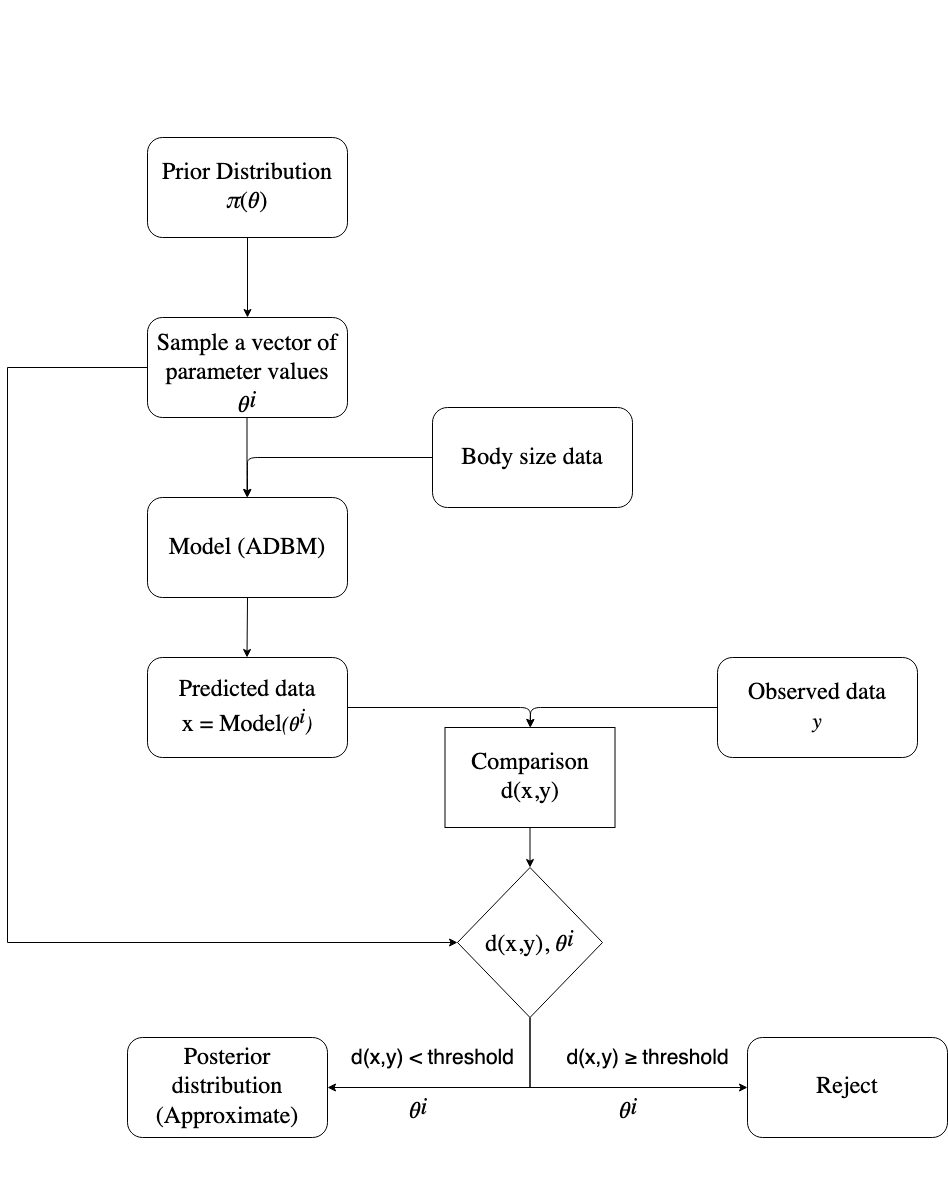
\includegraphics[width=400px]{fig/schematic} 

}

\caption{\label{fig:fig_m1} Flowchart of rejection approximate Bayesian computation method implemented to parameterise the ADBM.}\label{fig:unnamed-chunk-3}
\end{figure}

\hypertarget{prior-distribution}{%
\subsubsection{Prior distribution}\label{prior-distribution}}

The prior distributions for \(a_i\) and \(a_j\) were chosen to be
uniform distributions. The range of distribution was from -1.5 to 1.5
and 0 to 3 for \(a_i\) and \(a_j\) respectively, informed by the
estimates in Rall et al. (2012). However, we chose a prior range
specific to food webs for the parameter \(b\) because body size varies
greatly among the species in the observed food webs. For example: in the
Benguela Pelagic food web, the body sizes of species range from the
order of \(10^{-8}\) gm to \(10^5\) gm. Hence, the range of
prey-predator ratio was from the order of \(10^{-14}\) to \(10^{14}\).
To take this into account, we took the prior of \(log_{10}(b)\) from a
uniform distribution ranging from \(-15\) to \(15\).

For the prior of \(a\), we chose the prior of \(log_{10}(a)\) to be a
uniform distribution. Since, the ADBM estimated connectance to be higher
than the real connectance, lower values of \(a\) were favoured in the
parameterisation. Hence, the upper bound of the prior was set to 10. To
set the lower bound, we investigated how the true skill statistic varied
with \(log_{10}(a)\) (e.g.~SI Fig. S28). We found that the TSS increased
with decreasing \(log_{10}(a)\) and then remained constant, for a
constant value of \(log_{10}(b)\). We therefore decided to set the lower
bound of \(log_{10}(a)\) such that the maximum variation of TSS was
taken into account, while attempting to keep the range of prior as small
as possible. In the case of Benguela Pelagic as shown in SI Fig. S28,
the lower bound of \(log_{10}(a)\) was taken to be -12.

\hypertarget{comparison-of-observed-and-predicted}{%
\subsubsection{Comparison of observed and
predicted}\label{comparison-of-observed-and-predicted}}

The difference between the model's prediction and the observed data
(e.g.~the sum of squared residuals is such a distance in linear
regression) is quantified by a distance measure. The distance is lower
when there is a closer match between the model's prediction and the
observation. A perfect match would result in zero distance.

The magnitude of the distance is used for the acceptance or rejection of
a set of parameter values. An accepted set of parameter values
contributes to the posterior distribution, rejected ones do not. This
makes the distance measure one of the important features of ABC. A
threshold distance is chosen, and if the distance for a particular set
of parameter values is less than the threshold, then that set of
parameter values contributes to the posterior distribution. When the
distance is greater than the threshold, the parameter values do not
contribute to the posterior. Hence, the magnitude of the distance
threshold determines the proportion of a model's parameters that are
accepted. A higher threshold causes a high proportion of acceptances but
less accuracy with the acceptance of some parameter sets that result in
predictions quite unlike the observed data. Below, we first describe and
justify our choice of distance measure, and then our choice of
threshold.

\hypertarget{choice-of-distance-measure}{%
\paragraph{Choice of distance
measure}\label{choice-of-distance-measure}}

In the PBRW study the measure of distance was equivalent to
\(1 - TP / (TP + FN)\), where \(TP\) is the number of observed links
that were predicted (the number of true positives) and \(FN\) is the
number of observed links that were not predicted (the number of false
negatives). A distance of 0 indicates that all observed links were
correctly predicted. One way for the ADBM to achieve this is to predict
that every species has a trophic link with every other species including
itself -- a fully connected food web with connectance of 1. The PBRW
study prevented this by constraining the number of predicted links to be
equal to the number of observed links, i.e.~the model connectance was
fixed to be the same as the observed connectance. In this study, we
relaxed this constraint, with the number of links as well as the
arrangement of links being estimated. The first step was to choose an
appropriate distance measure.

The distance measure used in this study is 1 minus the true skill
statistic: \(\text{distance} = 1 - \text{TSS}\). This distance ranges
from 0 to 2.

TSS is defined as:

\[ \text{TSS} = \frac{TP\cdot TN- FP \cdot FN}{(TP+FN)(FP+TN)} \] where
\(TP\) is the number of observed links that are predicted by the model
(true positives), \(TN\) is the number of observed absences of links
that are correctly predicted (true negatives), \(FP\) is the number of
false positives, and \(FN\) is the number of false negatives.

The \(TSS\) ranges from \(-1\) to \(1\), where +1 indicates a perfect
prediction. A \(TSS\) value of zero or less indicates a performance no
better than random.

The inclusion of true and false negatives in the distance measure means
that the best theoretically possible prediction (smallest distance) is a
unique prediction, and specifically the one in which the predicted
presence and absence of links matches exactly with the observed presence
and absence of links.

\hypertarget{choice-of-threshold-value-of-distance}{%
\paragraph{Choice of threshold value of
distance}\label{choice-of-threshold-value-of-distance}}

Food web dynamics and stability are strongly dependent on connectance
(May 1972), we therefore set the distance threshold (for acceptance)
such that the model had a reasonable chance of predicting the observed
value of connectance. Note that in the following section (\emph{The
Rejection ABC method}) we use the term \(tol\) to denote the value of
the distance threshold.

To do this, we examined how the predicted connectance varied with the
distance threshold. An example of this relationship is given in Fig.
\ref{fig:fig_m2} for the Benguela Pelagic food web and in SI. Fig. S1
for other food webs. We chose the minimum threshold value that gave a
range of predicted connectance containing the observed connectance.

Furthermore, it is useful to note that in Fig. \ref{fig:fig_m2} there
are no connectance values below a distance threshold value of less than
0.5 because for this particular food web there were no sets of parameter
values that achieved a better model fit than is indicated by
\(1-TSS = 0.5\). I.e. it is impossible for the ADBM to make better
predictions than this. One reason for this is that the ADBM, when body
size is the only trait, can only predict contiguous diets in trait
space, whereas the observed data contains gaps in the diet.

\begin{figure}[h]

{\centering 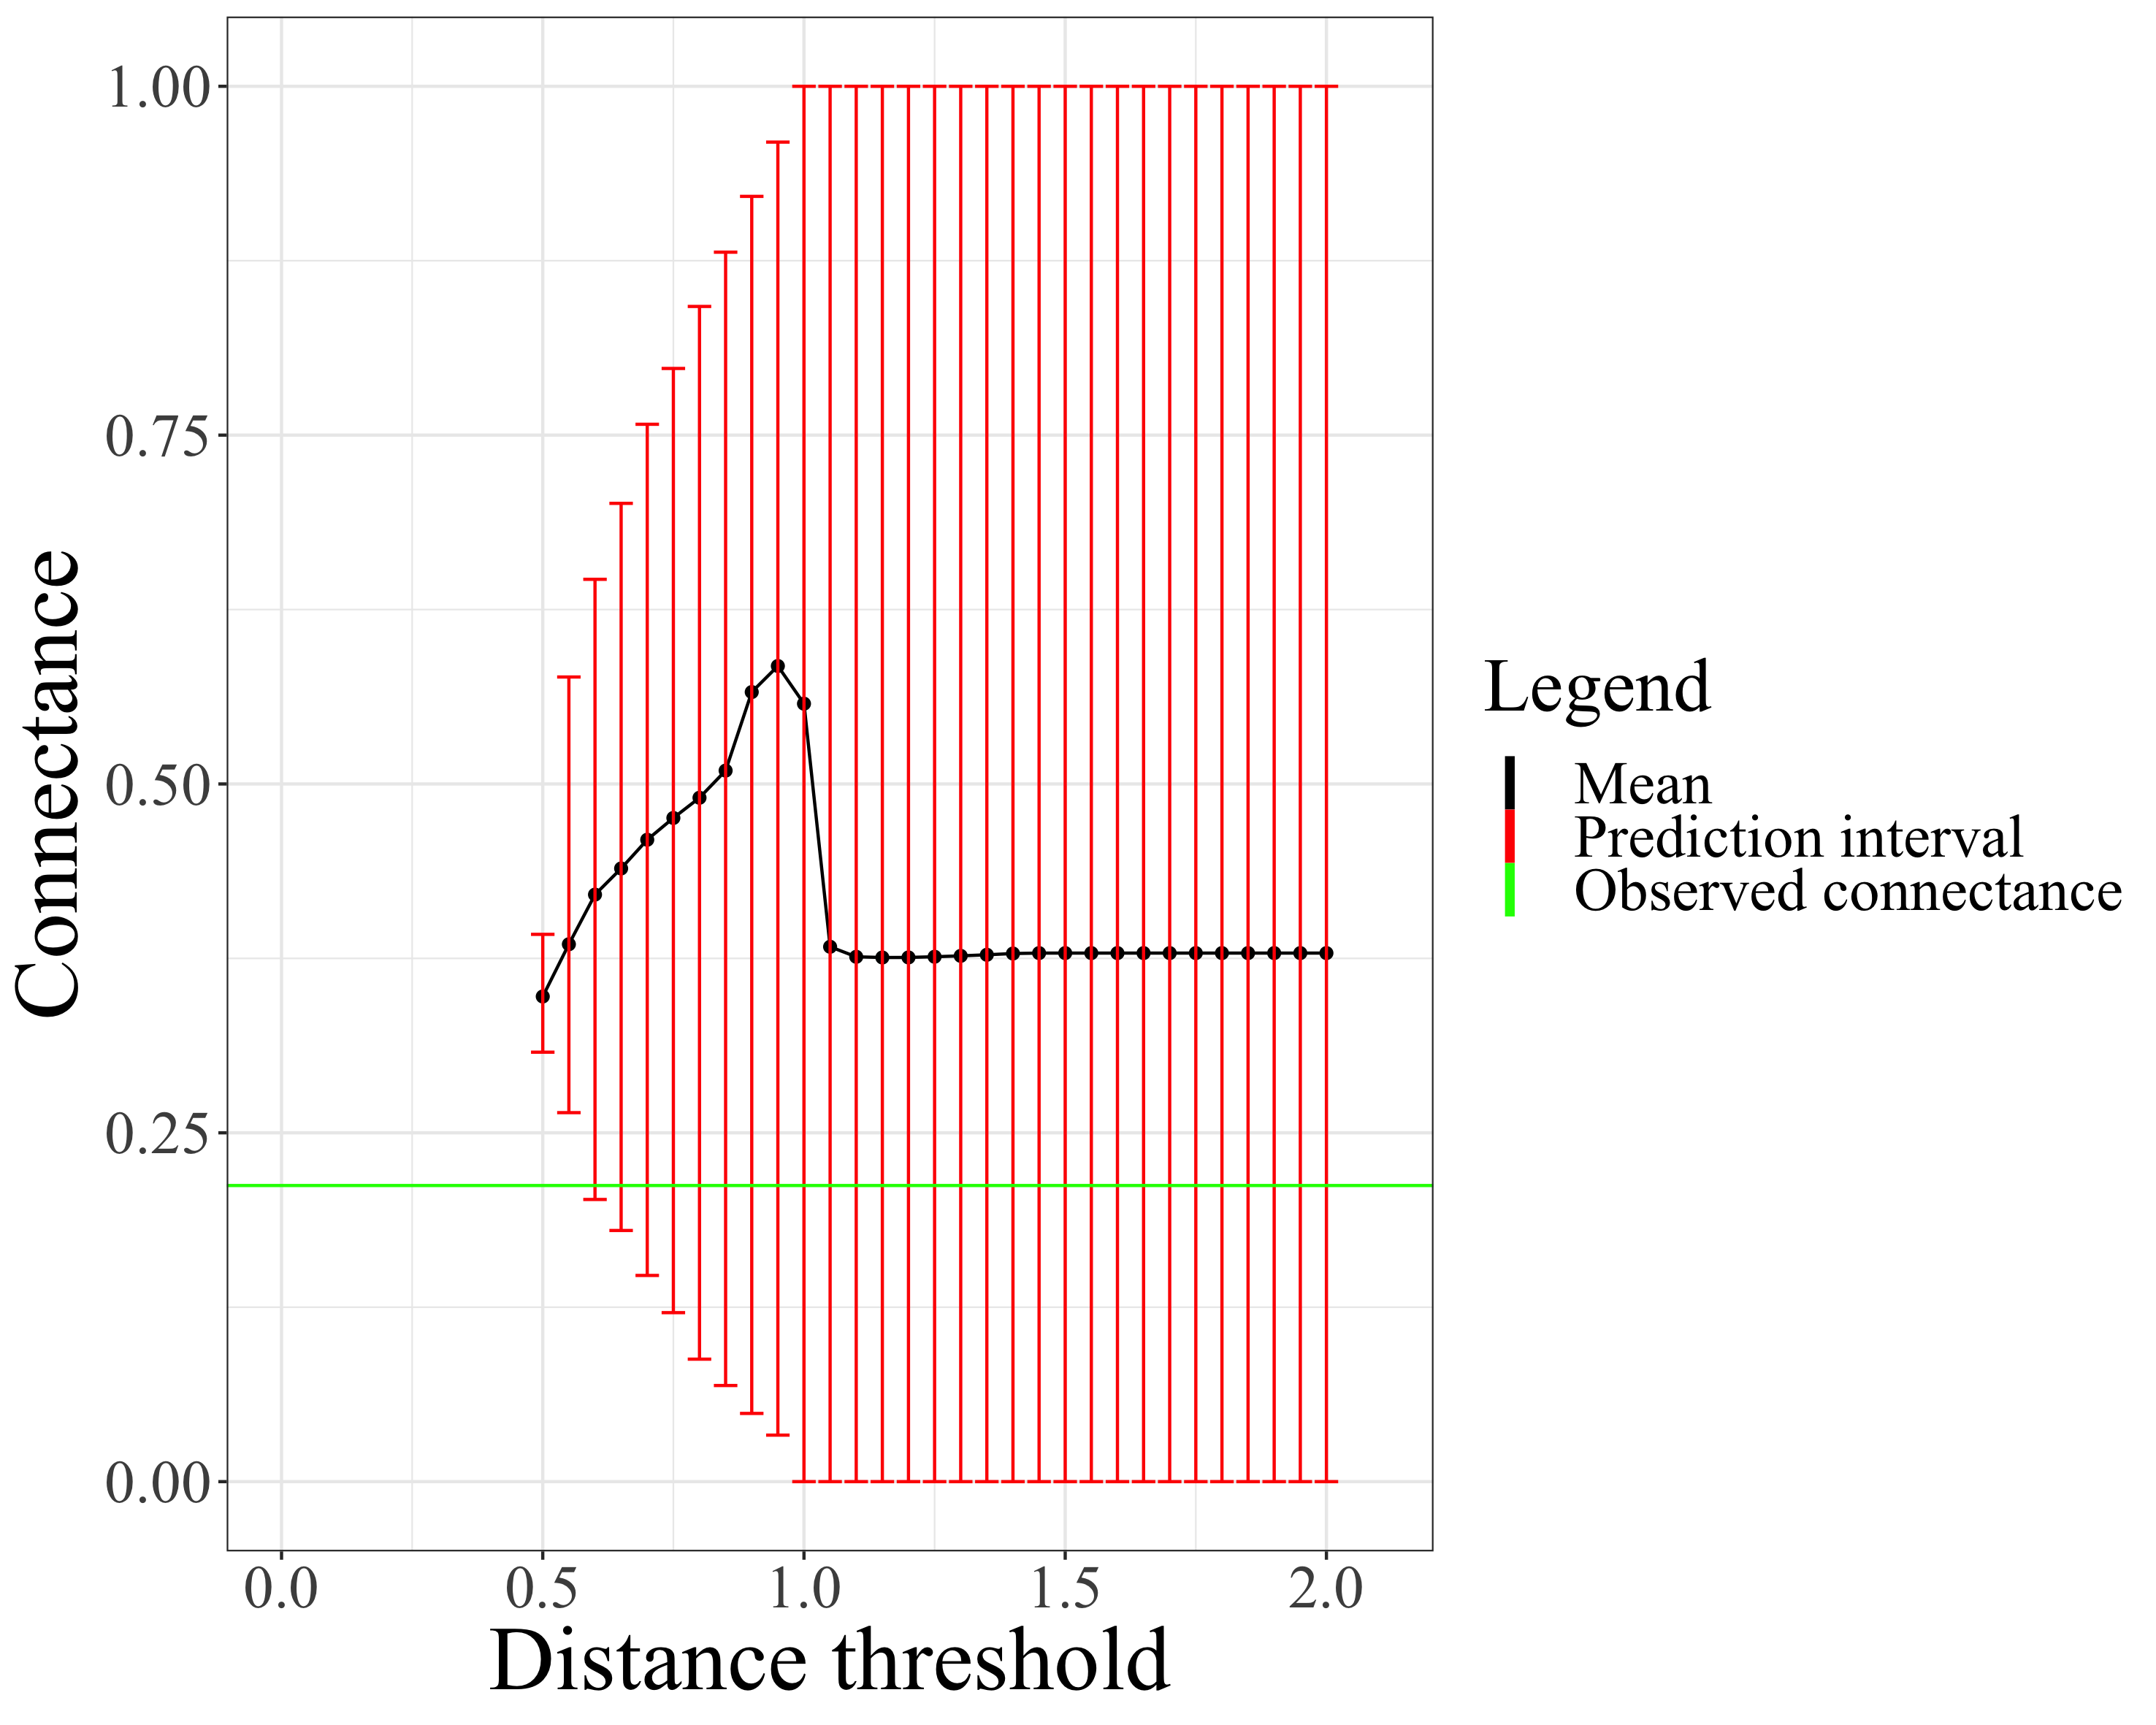
\includegraphics[width=300px]{fig/Benguela_Pelagic_connectanceCI_vs_tol} 

}

\caption{\label{fig:fig_m2}The prediction interval of the predicted connectance increases with increasing distance threshold for the Benguela Pelagic food web. The green line and black line represent the observed connectance and mean of predicted connectance respectively.}\label{fig:unnamed-chunk-4}
\end{figure}

\hypertarget{the-rejection-abc-method}{%
\subsubsection{The Rejection ABC
method}\label{the-rejection-abc-method}}

In the rejection ABC method, a set of parameter values are sampled from
the prior distributions. This set of parameter values is either
accepted, and thereby added to the posterior distribution of the
parameter values, or it is rejected (based on if the distance 1 -
\(TSS\) is less than or greater than the threshold distance, as
mentioned above). This process is repeated until there are enough
acceptances to give stable (approximate) posterior distributions.
Acceptance or rejection of a set of parameter values is probabilistic
and depends on a weight assigned to that set of parameter values. This
weight is given by a kernel function, where the weight is inversely
proportional to the distance (1 - \(TSS\)). This weight is then used in
a way that makes it the probability of the set of parameter values being
accepted.

In the upcoming section, we further detail the rejection ABC method.

\emph{Properties:}

\begin{itemize}
\item
  A prior distribution \(\pi(\theta)\): \(\pi\) is the uniform
  distribution for parameters \(\theta = (a, a_i, a_j, b)\)
\item
  A model prediction \(model(\theta)\): ADBM\((\theta)\). This is a
  predicted food web, \(x_i\), given by a particular set of parameter
  values \(\theta_i\). Hence, \(x_i = ADBM(\theta_i)\)
\item
  A summary statistic \(s(x)\): \(x\) is the predation matrix predicted
  by the ADBM.
\item
  \(\begin{aligned} \text{A kernel function } K(u): \text{ epanechnikov } K(u) &= \frac{1}{tol}\cdot\frac{3}{4}(1-(\frac{u}{tol})^2) \text{ if } u \leq tol \\ &= 0 \text{ otherwise} \end{aligned}\)
\end{itemize}

where \(tol\) is the distance threshold

\begin{itemize}
\item
  A distance function \(d(x_i,y)\): \(d(x_i,y) = 1 - TSS(x_i,y)\)
\item
  An observed food web \(y\), in the form of a predation matrix
  containing zeros and ones.
\end{itemize}

\emph{Sampling:}

for \(i = 1 \dots n = 1000\)

\begin{itemize}
\item
  Draw a set of parameter values \(\theta_i\) from the prior
  distribution \(\pi(\theta)\).
\item
  Compute the model result \(x_i = model(\theta_i)\)
\item
  Compute \(s(x_i)\) and \(d(s(x_i), s(y))\)
\item
  Accept or reject the parameter set probabilistically:

  \begin{itemize}
  \item
    Assign a weight \(p_i\) to \(\theta_i\) as per the kernel \(K\);
    \(p_i = \frac{K(d)}{K(0)}\), where \(d\) is the distance evaluated
    in the previous step.
  \item
    Compute \(\alpha \sim U(0,1)\)
  \item
    If \(\alpha \leq p_i\), then accept \(\theta_i\) and \(i = i + 1\)
  \end{itemize}
\end{itemize}

\emph{Output:}

An approximate joint posterior distribution using the accepted
\(\theta_1, \dots, \theta_n\).

\hypertarget{assessment-of-model-fit}{%
\subsection{Assessment of model fit}\label{assessment-of-model-fit}}

Accuracy is how close the model prediction is to the observation. The
ADBM's prediction is a predation matrix that consists of the presence
and absence of links thus comparing how close the prediction is to the
observation is not straightforward as comparing two numerical values. We
defined the accuracy of the ADBM using true skill statistics to take
into account the true and false predictions of both the presence and
absence of links, which is defined above.

We examined how closely structural properties of the predicted food web
matched those of the observed food webs using the R \emph{cheddar}
package (Hudson et al. 2013). We evaluated properties such as proportion
of basal species, proportion of intermediate species, proportion of top
species, proportion of herbivores, mean omnivory, clustering
coefficient, standard deviation of generality, standard deviation of
vulnerability, diet similarity, mean path length and nestedness. We
could not compute mean trophic level and maximum trophic level because
the networks contained too many paths for the \emph{cheddar} package
algorithm to compute.

We investigated the performance of the ADBM parameterised with the ABC
by computing standardised error of the food web properties, where the
standardised error is the absolute raw error (the difference between
observed and predicted value) divided by the maximum absolute raw error
for that property. We did not calculate the standardised error for mean
omnivory and mean path length because it had some NA values and infinite
values for all the food webs respectively.

\hypertarget{results}{%
\section{Results}\label{results}}

As an example of the model outcomes, we first present the results for
the Benguela food web (e.g.~predicted food web structure, variation in
predicted food web structure, and posterior parameter distributions). We
chose this food web as it was well explained using the method of
(Petchey et al. 2008) (hereafter referred as PBRW study). The results of
the other food webs are included in the SI Figs S2-S25. We then compare
model outcomes across all empirical food webs between the PBRW study and
our current work. We compare the true skill statistic of the two
approaches and compare some food web properties, such as proportions of
basal, intermediate, and top species.

The true skill statistic (TSS) of the predicted Benguela Pelagic food
web varied between 0.4 and 0.52. This variation in the TSS is
represented in terms of predation matrices displayed in Fig.
\ref{fig:fig_r1}(a), which overlays 1000 independent predation matrices
accepted from the ABC method. In all the 1000 independent predation
matrices, the predicted links are mostly present in the upper triangular
portion of the matrix where most of the observed links are also present.
Links in the upper right triangle of the predation matrix are for
predators feeding on prey smaller than themselves.

In the 1000 predicted predation matrices, there predators are sometimes
smaller than their predicted prey, the links in the lower left triangle
of the predation matrix. This is also portrayed in the marginal
distribution of \(log_{10}(b)\) in Fig. \ref{fig:fig_r3}(d), as it
includes values greater than \(b=2\) (\(log_{10}(b)=0.3\)). This is
relevant as values of \(b=2\) make the most profitable prey item equal
in size to the predator size. Lower values of \(b\) make the most
profitable prey item smaller than the size of the predator.

There were around 250 potential links in the lower left triangle of the
predation matrix that were never predicted in any of the 1000 predicted
predation matrix (Fig. \ref{fig:fig_r1}(b)). This strongly suggests that
the predator-prey size ratio of these links is so small (i.e.~very large
prey, very small predator) that the links cannot occur, given that the
preponderance of observed links are predators consuming prey smaller
than themselves.

\begin{figure}

{\centering 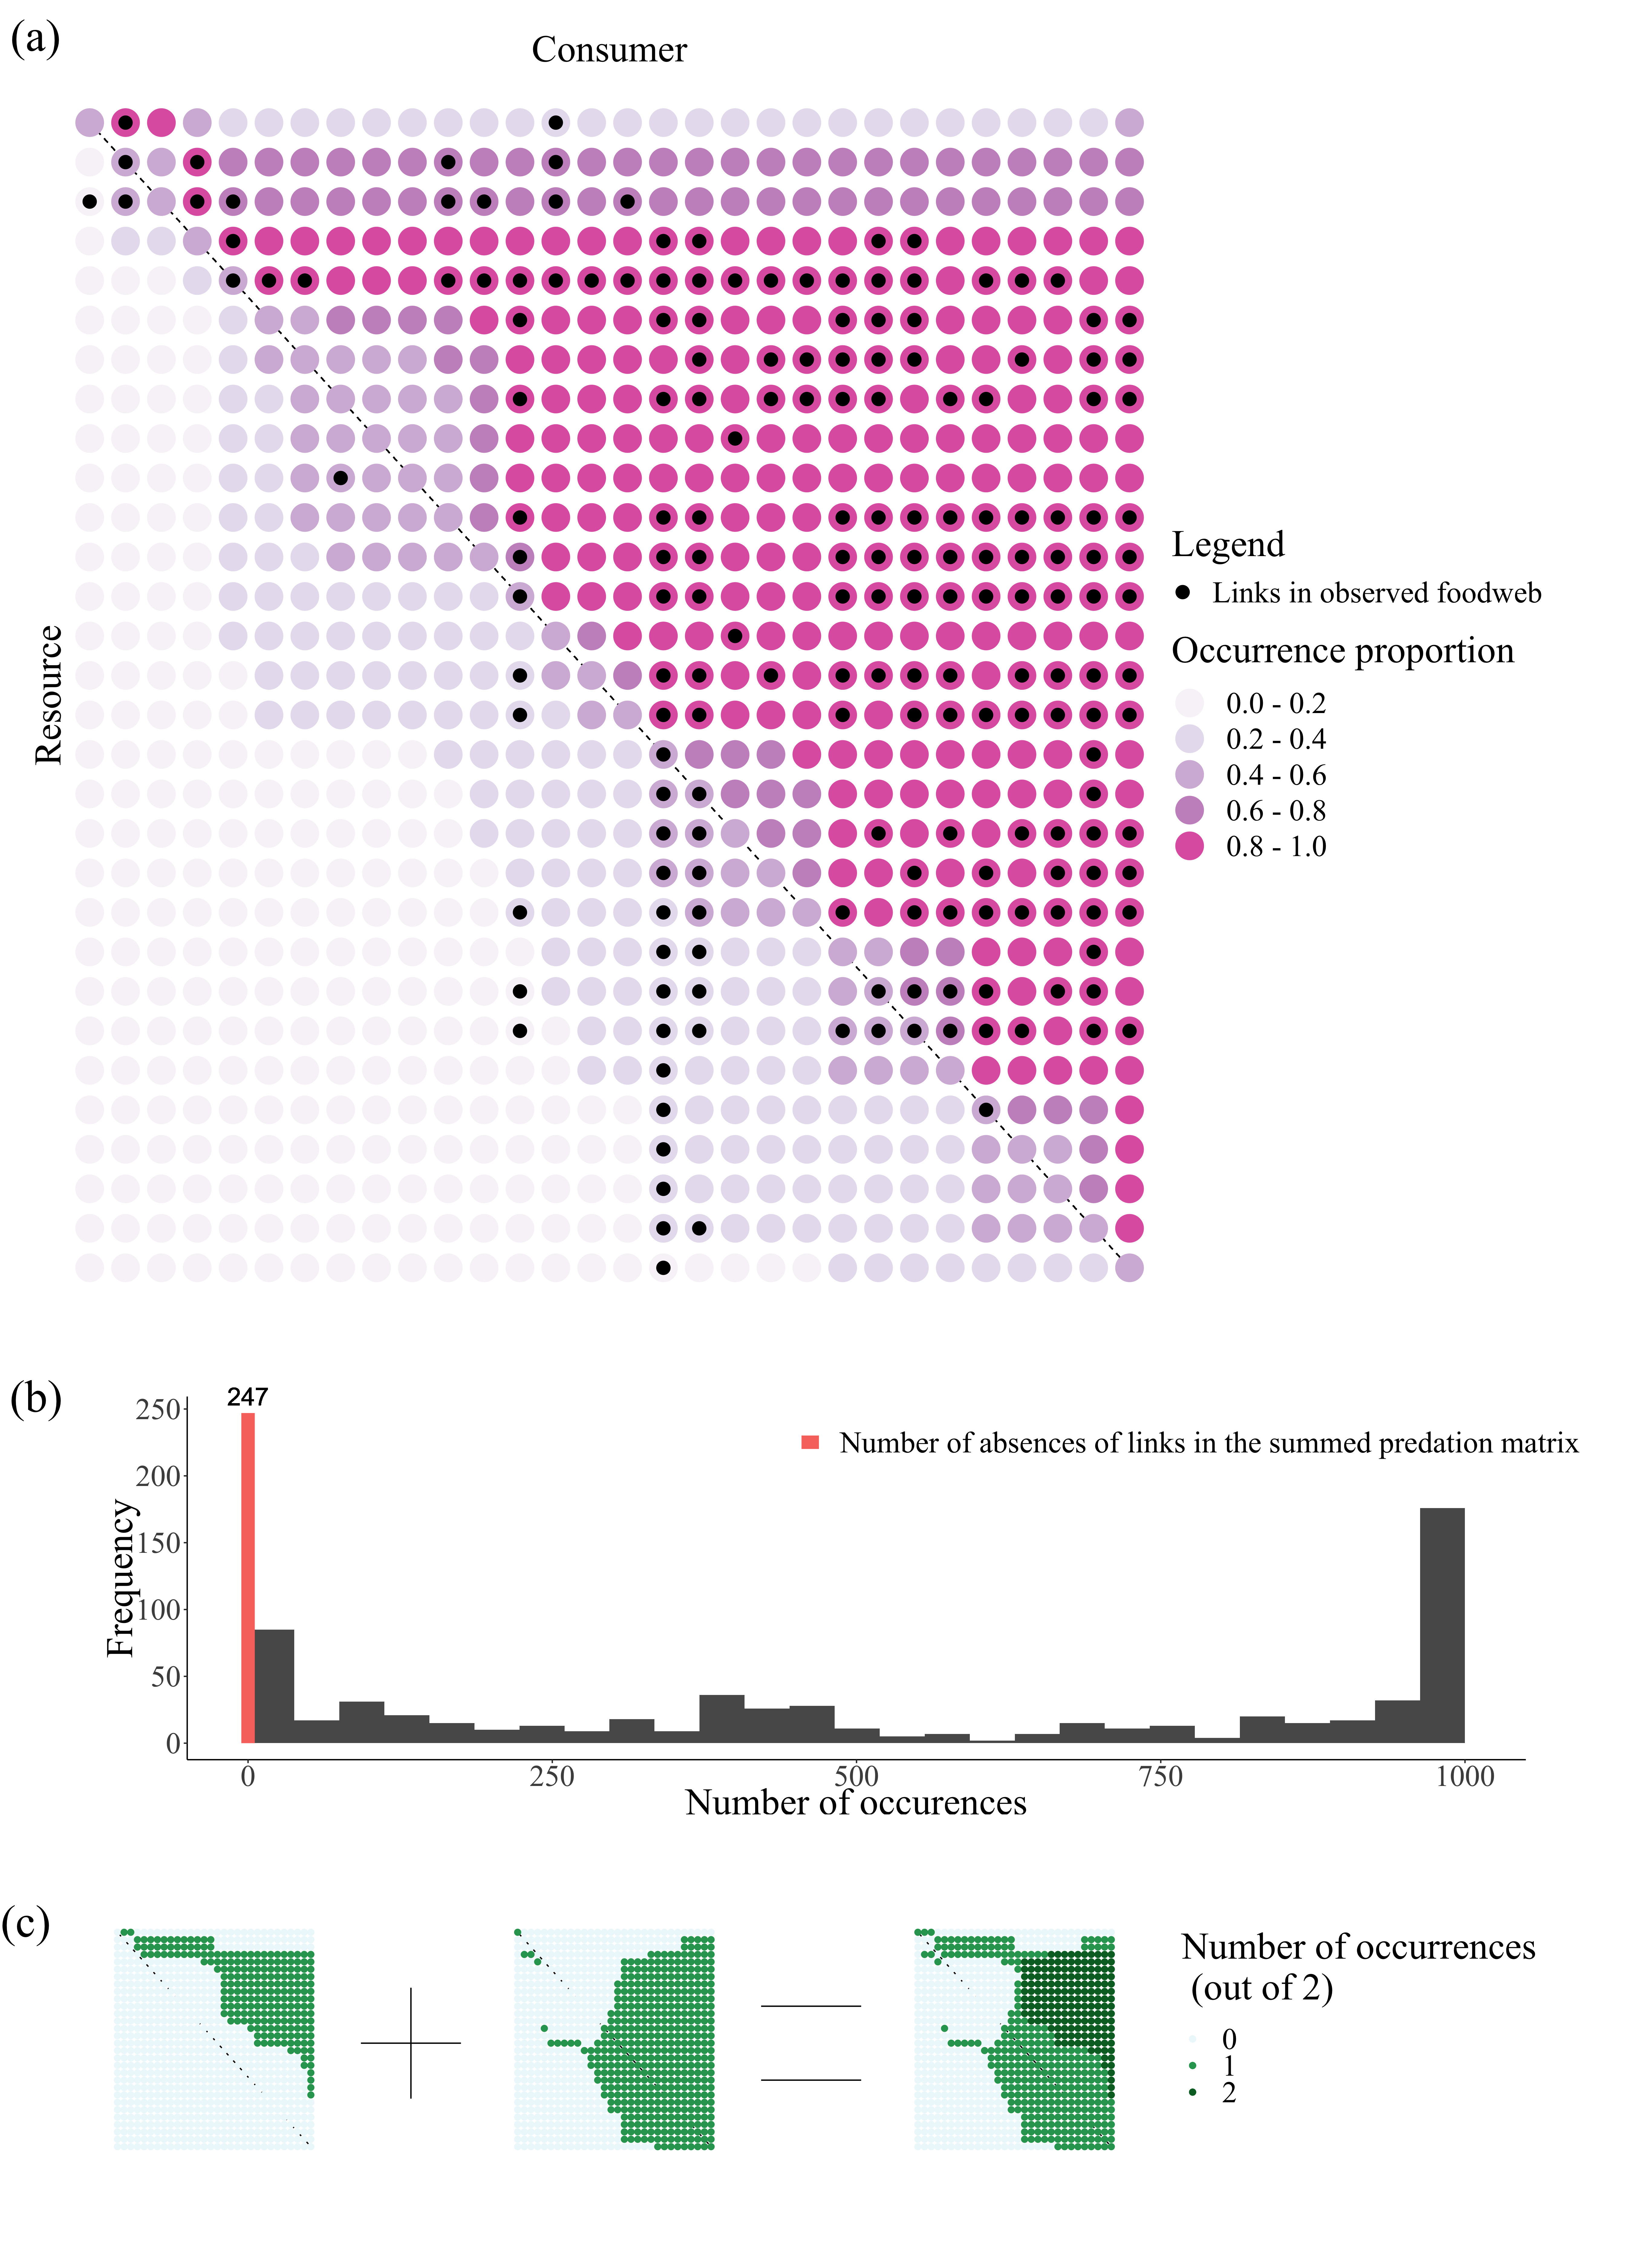
\includegraphics[width=300px]{fig/Benguela_Pelagic_pred_mat} 

}

\caption{\label{fig:fig_r1} (a) Observed and predicted predation matrices for Benguela Pelagic food web. Body size increases from left to right and top to bottom along the predation matrix. Black circles show where there is an observed trophic link. The intensity of the pink circles shows the proportion of 1000 predicted food webs that had a trophic link between the corresponding species. This type of overlay is shown for two examples predicted in panel (c). (b) The histogram of the number of times a link was predicted across 1000 independently predicted food webs. There were 841 species pairs in this food web. About 150 of these were predicted to have a trophic link in all 1000 predicted predation matrices. The red bar shows the number of pairs of species for which a trophic link was never predicted. (c) Two predicted predation matrices for Benguela Pelagic food web corresponding to the minimum and the maximum value of estimated $b$, and their sum.}\label{fig:unnamed-chunk-5}
\end{figure}

The marginal posterior of parameter \(b\) in the Benguela Pelagic food
web was more constrained than the marginal posterior distribution of the
other three allometric parameters (Fig. \ref{fig:fig_r3}) as the
posterior range was the narrowest.

\begin{figure}

{\centering 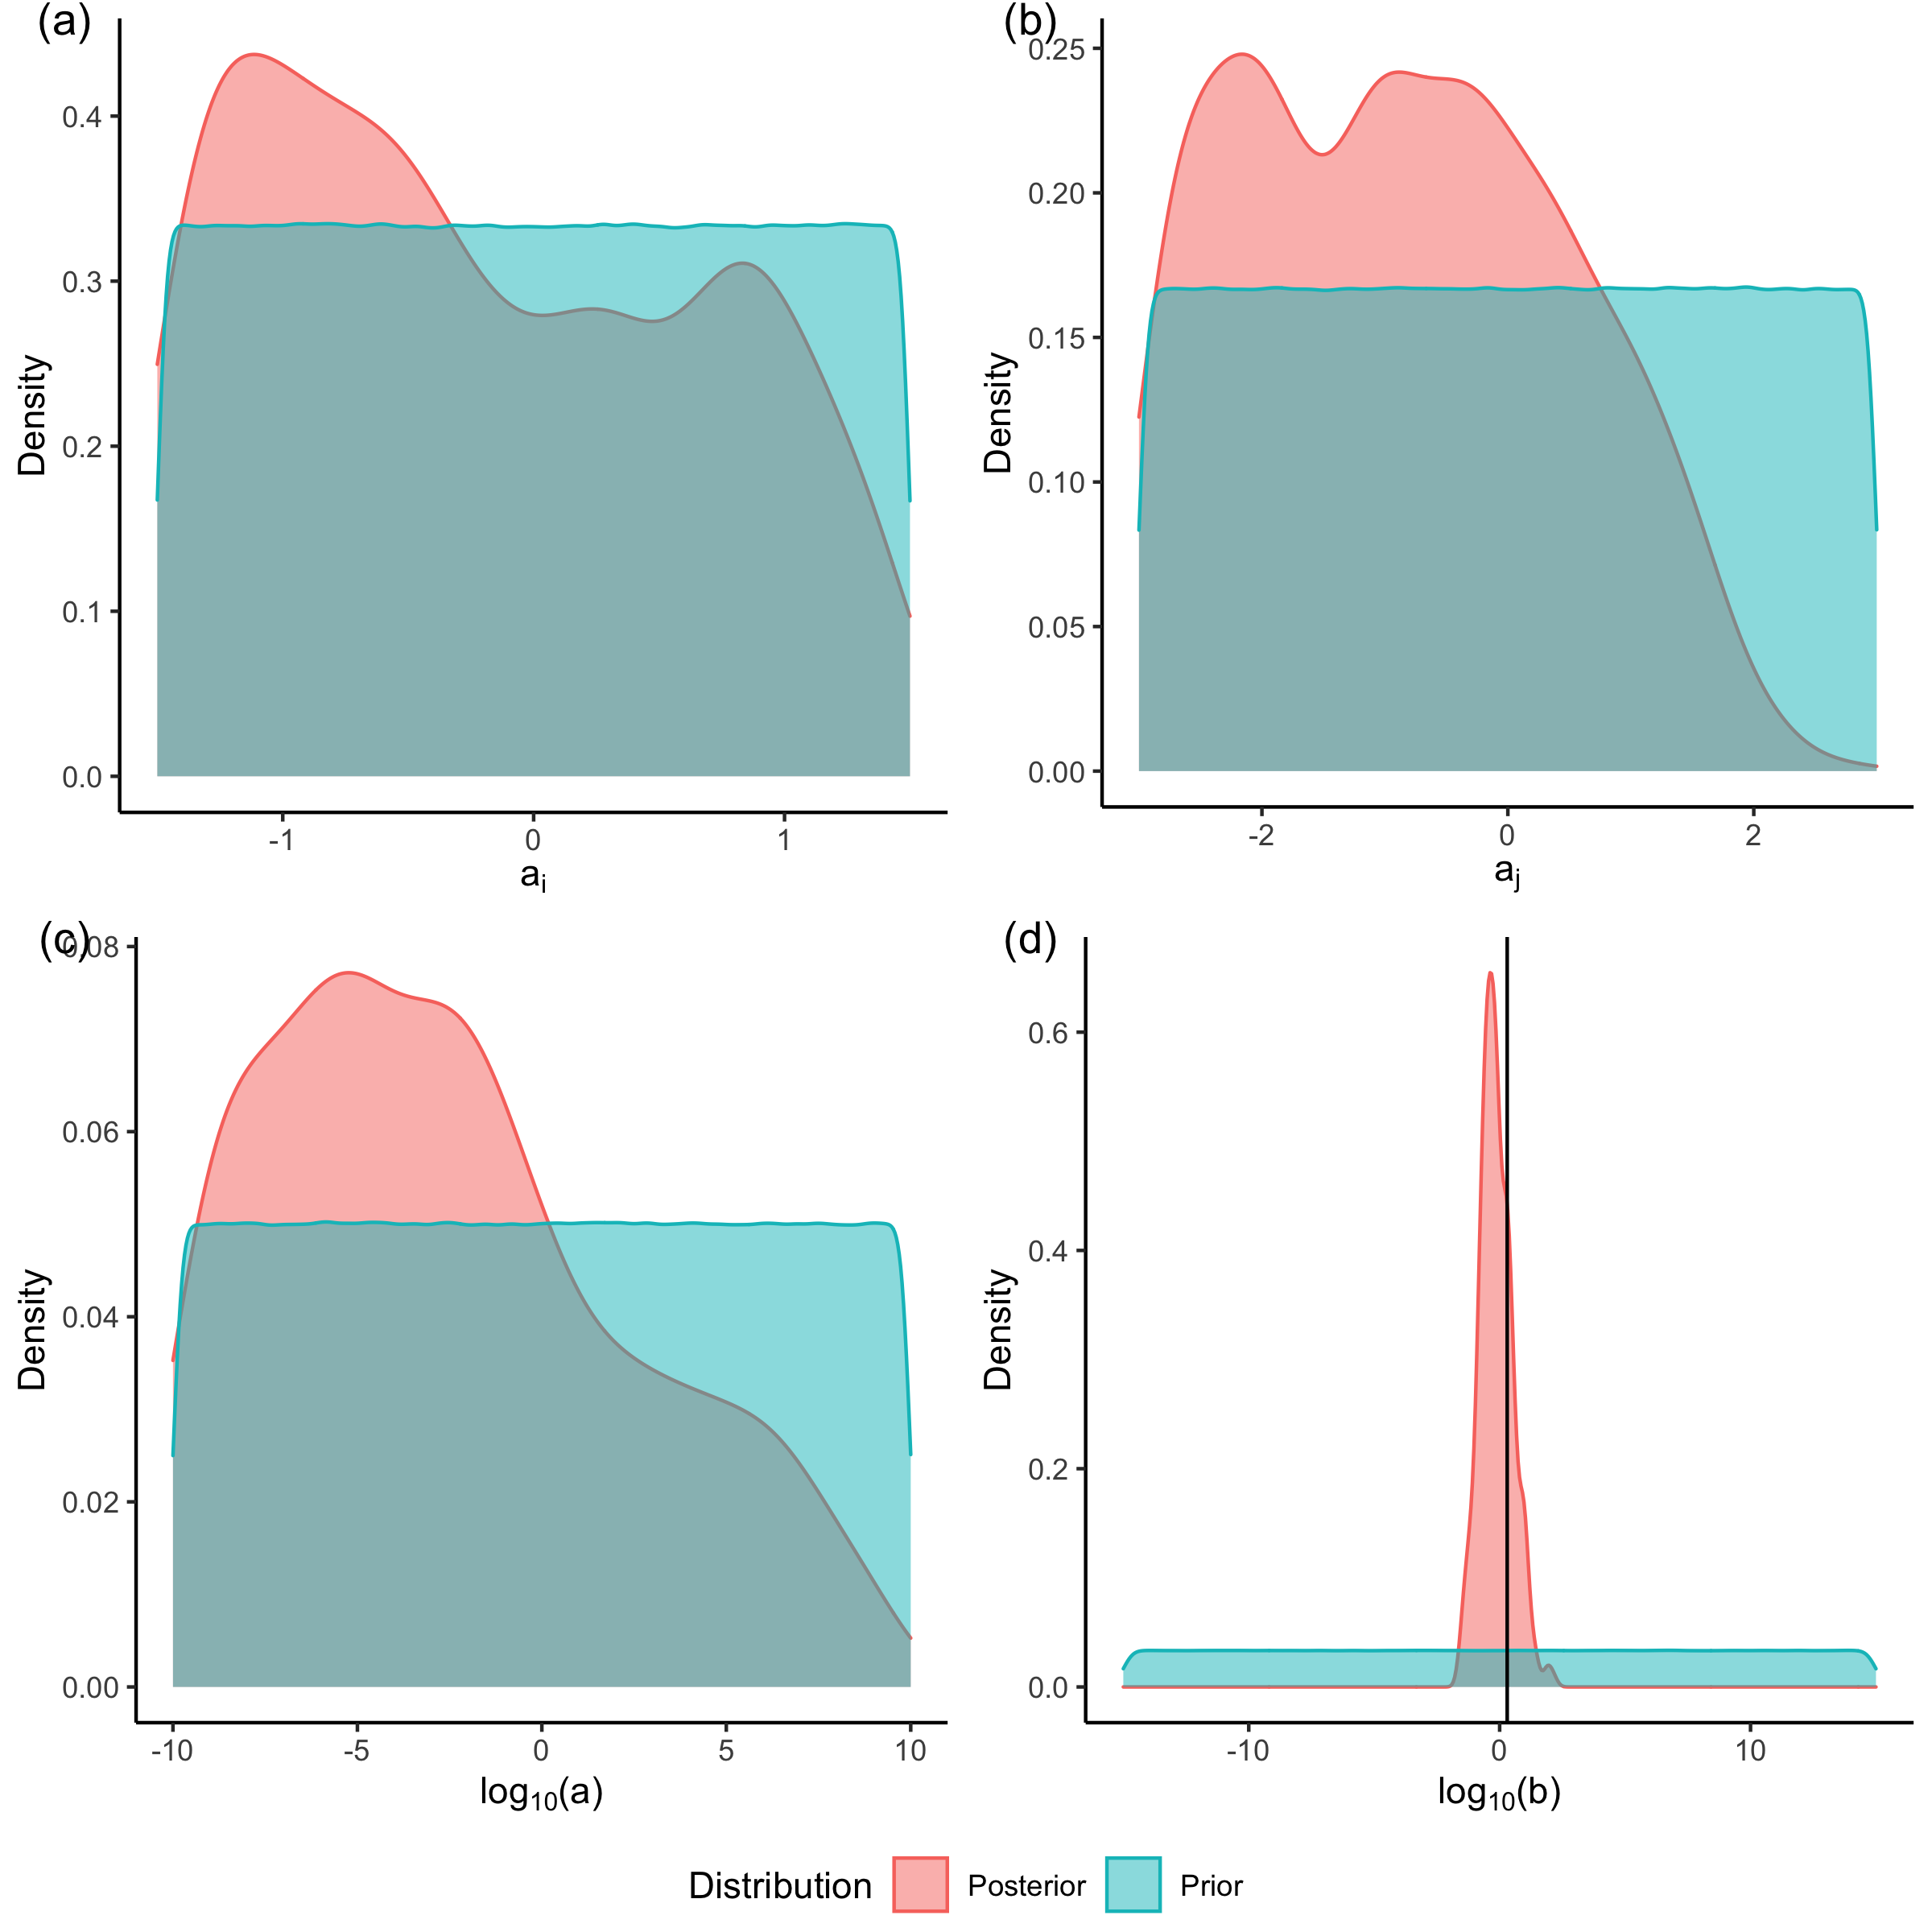
\includegraphics[width=300px]{fig/Benguela_Pelagic_distribution} 

}

\caption{\label{fig:fig_r3} Marginal prior and marginal posterior distribution of the ADBM parameters for the Benguela Pelagic food web estimated using rejection ABC. The black vertical line in (d) corresponds to the value of $b$ (=2) above which the most profitable prey item is larger in respect to the predator size.}\label{fig:unnamed-chunk-6}
\end{figure}

\begin{figure}

{\centering 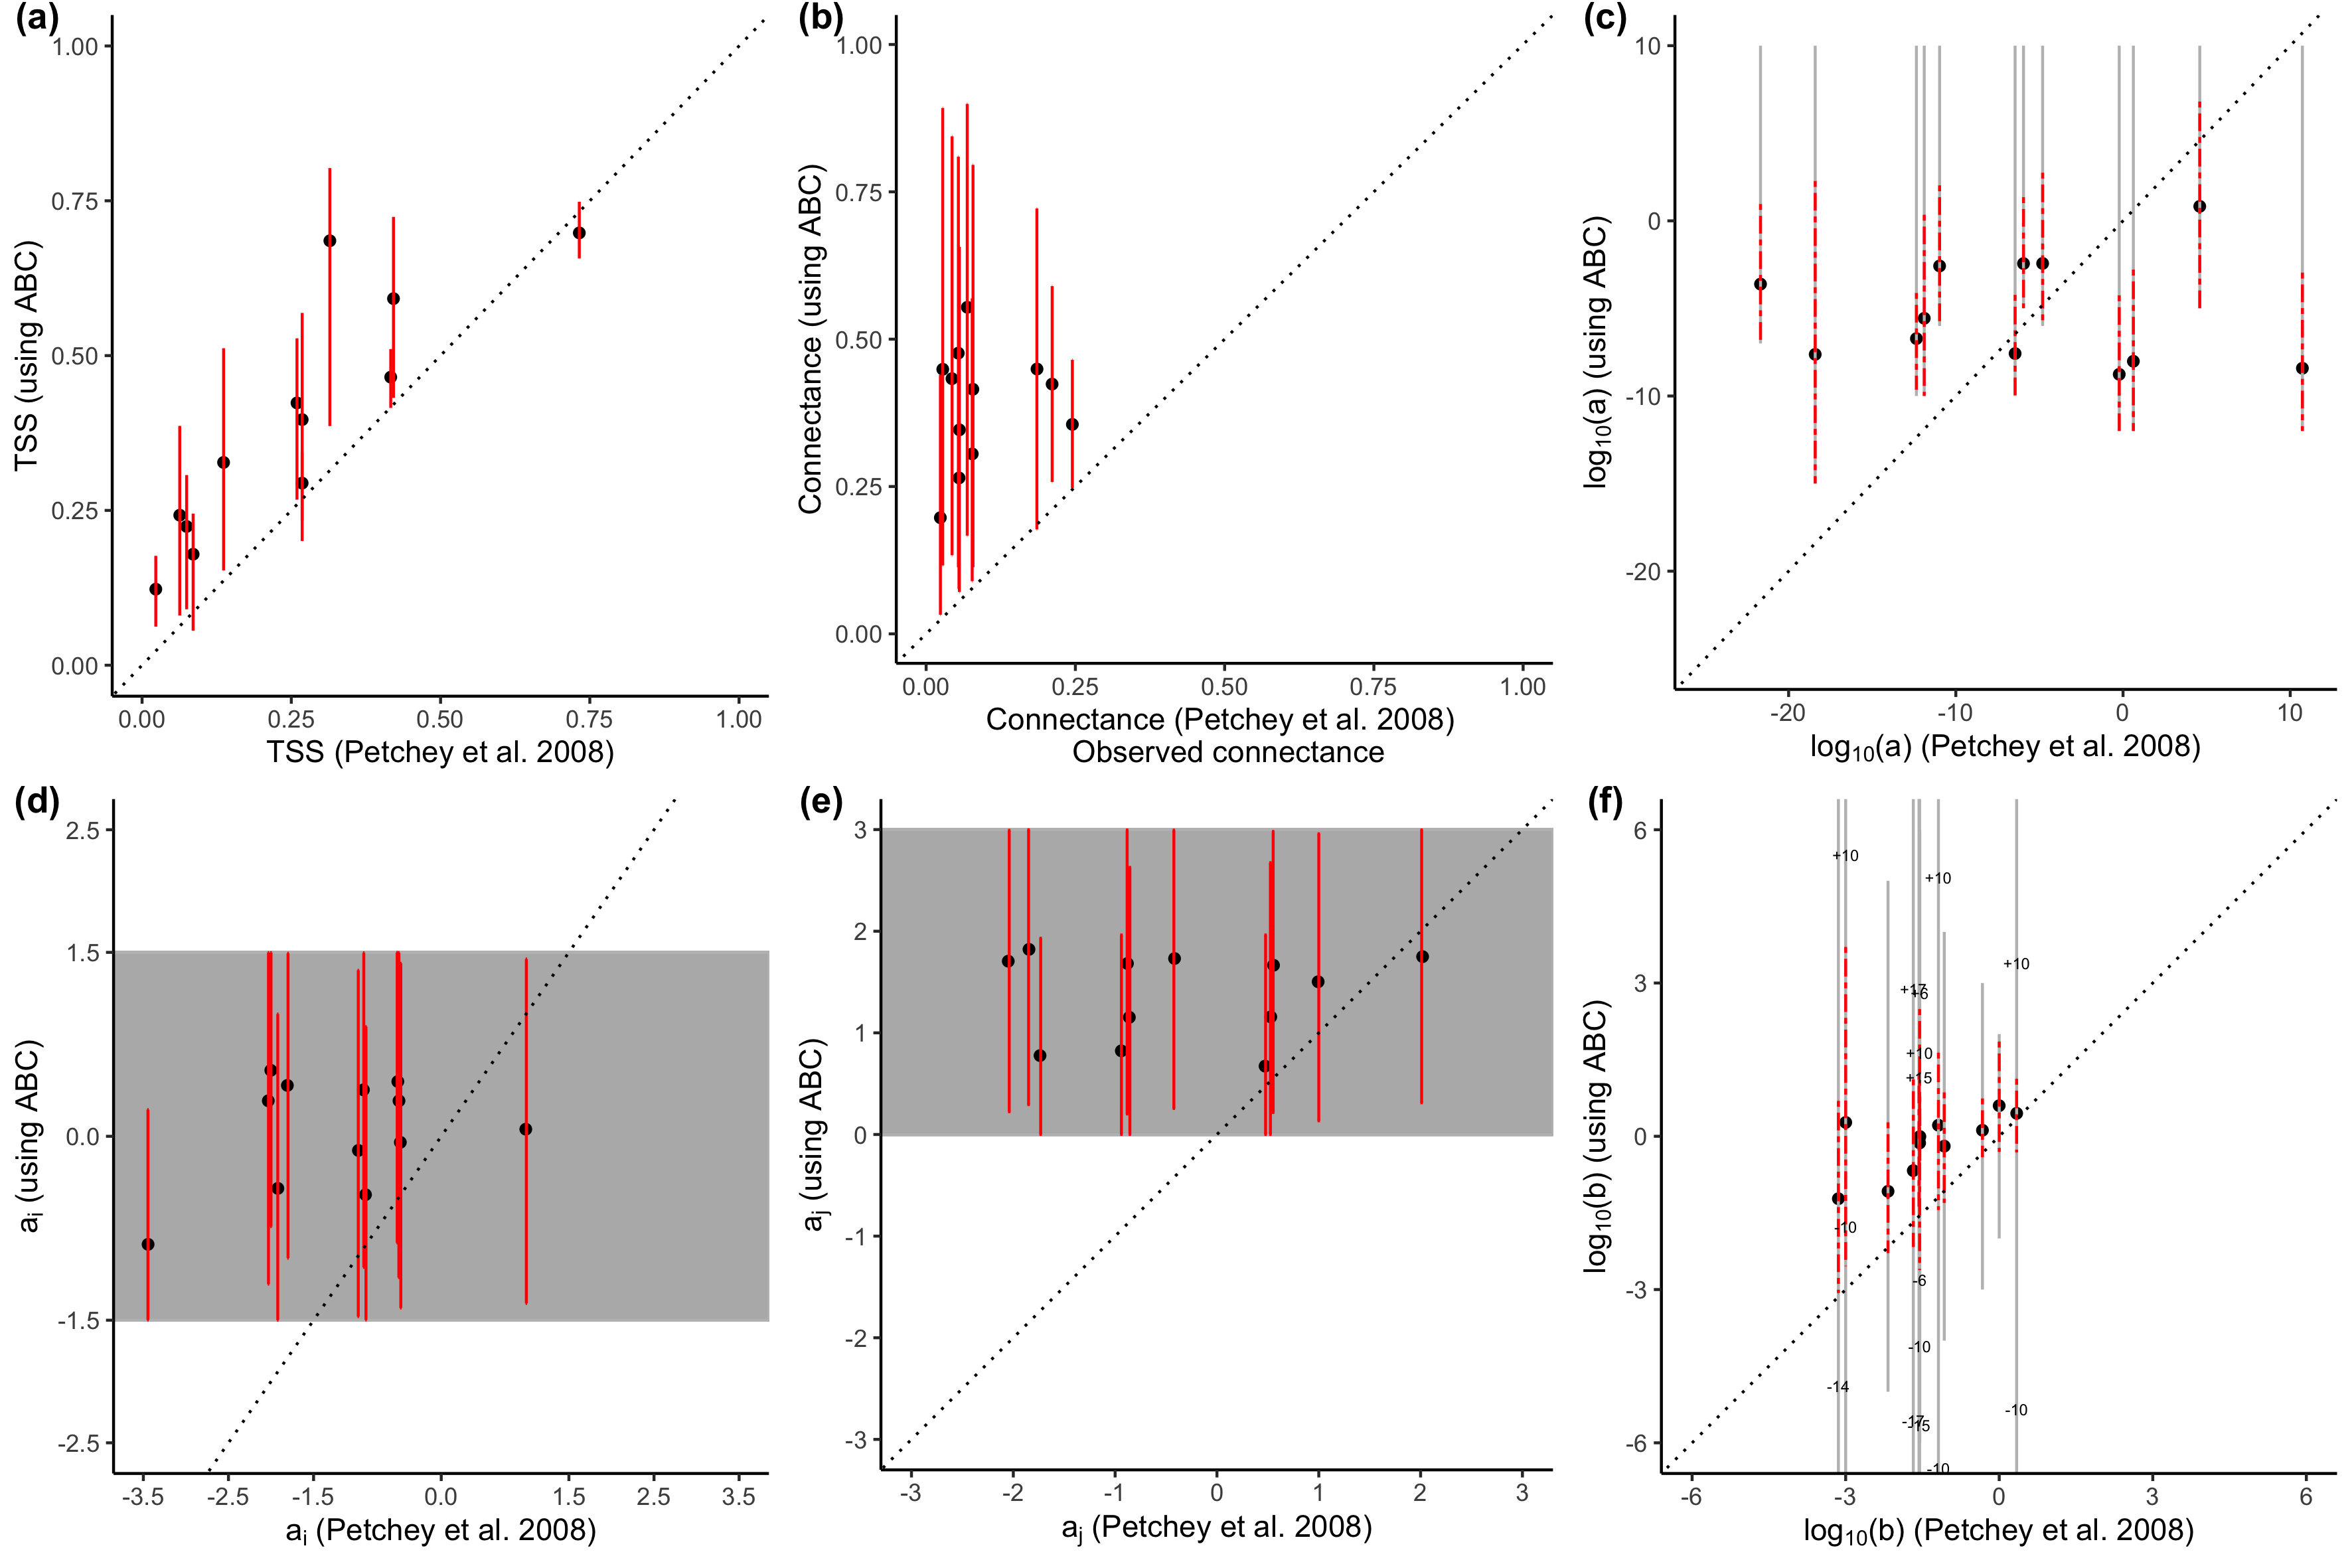
\includegraphics[width=500px]{../results/misc/ABC_vs_point_estimates} 

}

\caption{\label{fig:fig_r2} TSS (a), connectance (b) and ADBM parameters (c, d, e, f) computed using the ABC method compared with the corresponding point estimates from Petchey et al. (2008). The red lines are the 95\% credible/prediction intervals and the black filled circles represent the corresponding means. The grey region represents the intervals of the prior distributions for $a_i$ and $a_j$. The grey lines represent the prior range of the parameters $a$ and $b$ in the $log_{10}$ scale. The prior range for the parameter $b$ extends above and below the y-axis limits for some food webs and so the values of the limits are shown on the plot. The dashed black lines are the 1:1 relationships for reference.}\label{fig:unnamed-chunk-7}
\end{figure}

The mean true skill statistic using the ABC approach was higher than the
point estimates from the PBRW study (Fig. \ref{fig:fig_r2}(a)) across
all food webs except one. Our present approach led to estimates of
connectance greater than the values of connectance of the PBRW study,
which were fixed to equal the observed values of connectance.

We did not find a consistent relationship between the parameters
estimated using the current approach and those estimated in the PBRW
study (Fig. \ref{fig:fig_r2}(c-f)), except for in the case of parameter
\(b\). The mean using the ABC approach was always higher than the
estimates from the PBRW study (Fig. \ref{fig:fig_r2}(f)) and the 95\%
credible interval of the posterior of \(b\) includes the estimate from
the PBRW study.

The marginal posterior of parameter \(b\) was more constrained than the
other three allometric parameters, i.e.~the posterior range was the
narrowest (SI Figs S14-S25). In all of the food webs except Grasslands,
the parameter \(b\) had a unimodal distribution (SI Figs S14-S25)
whereas Grasslands had a bimodal distribution.

The structural food web properties proportion of intermediate species,
mean omnivory, clustering coefficient, sd of generality, sd of
vulnerability, diet similarity and nestedness estimated from the current
ABC approach were generally higher than the PBRW study (Fig.
\ref{fig:fig_r4p5}(b, e-j)). The properties proportion of basal species,
proportion of top species, and proportion of herbivores were generally
lower (Fig. \ref{fig:fig_r4p5}(a, c, d)).

\begin{figure}

{\centering 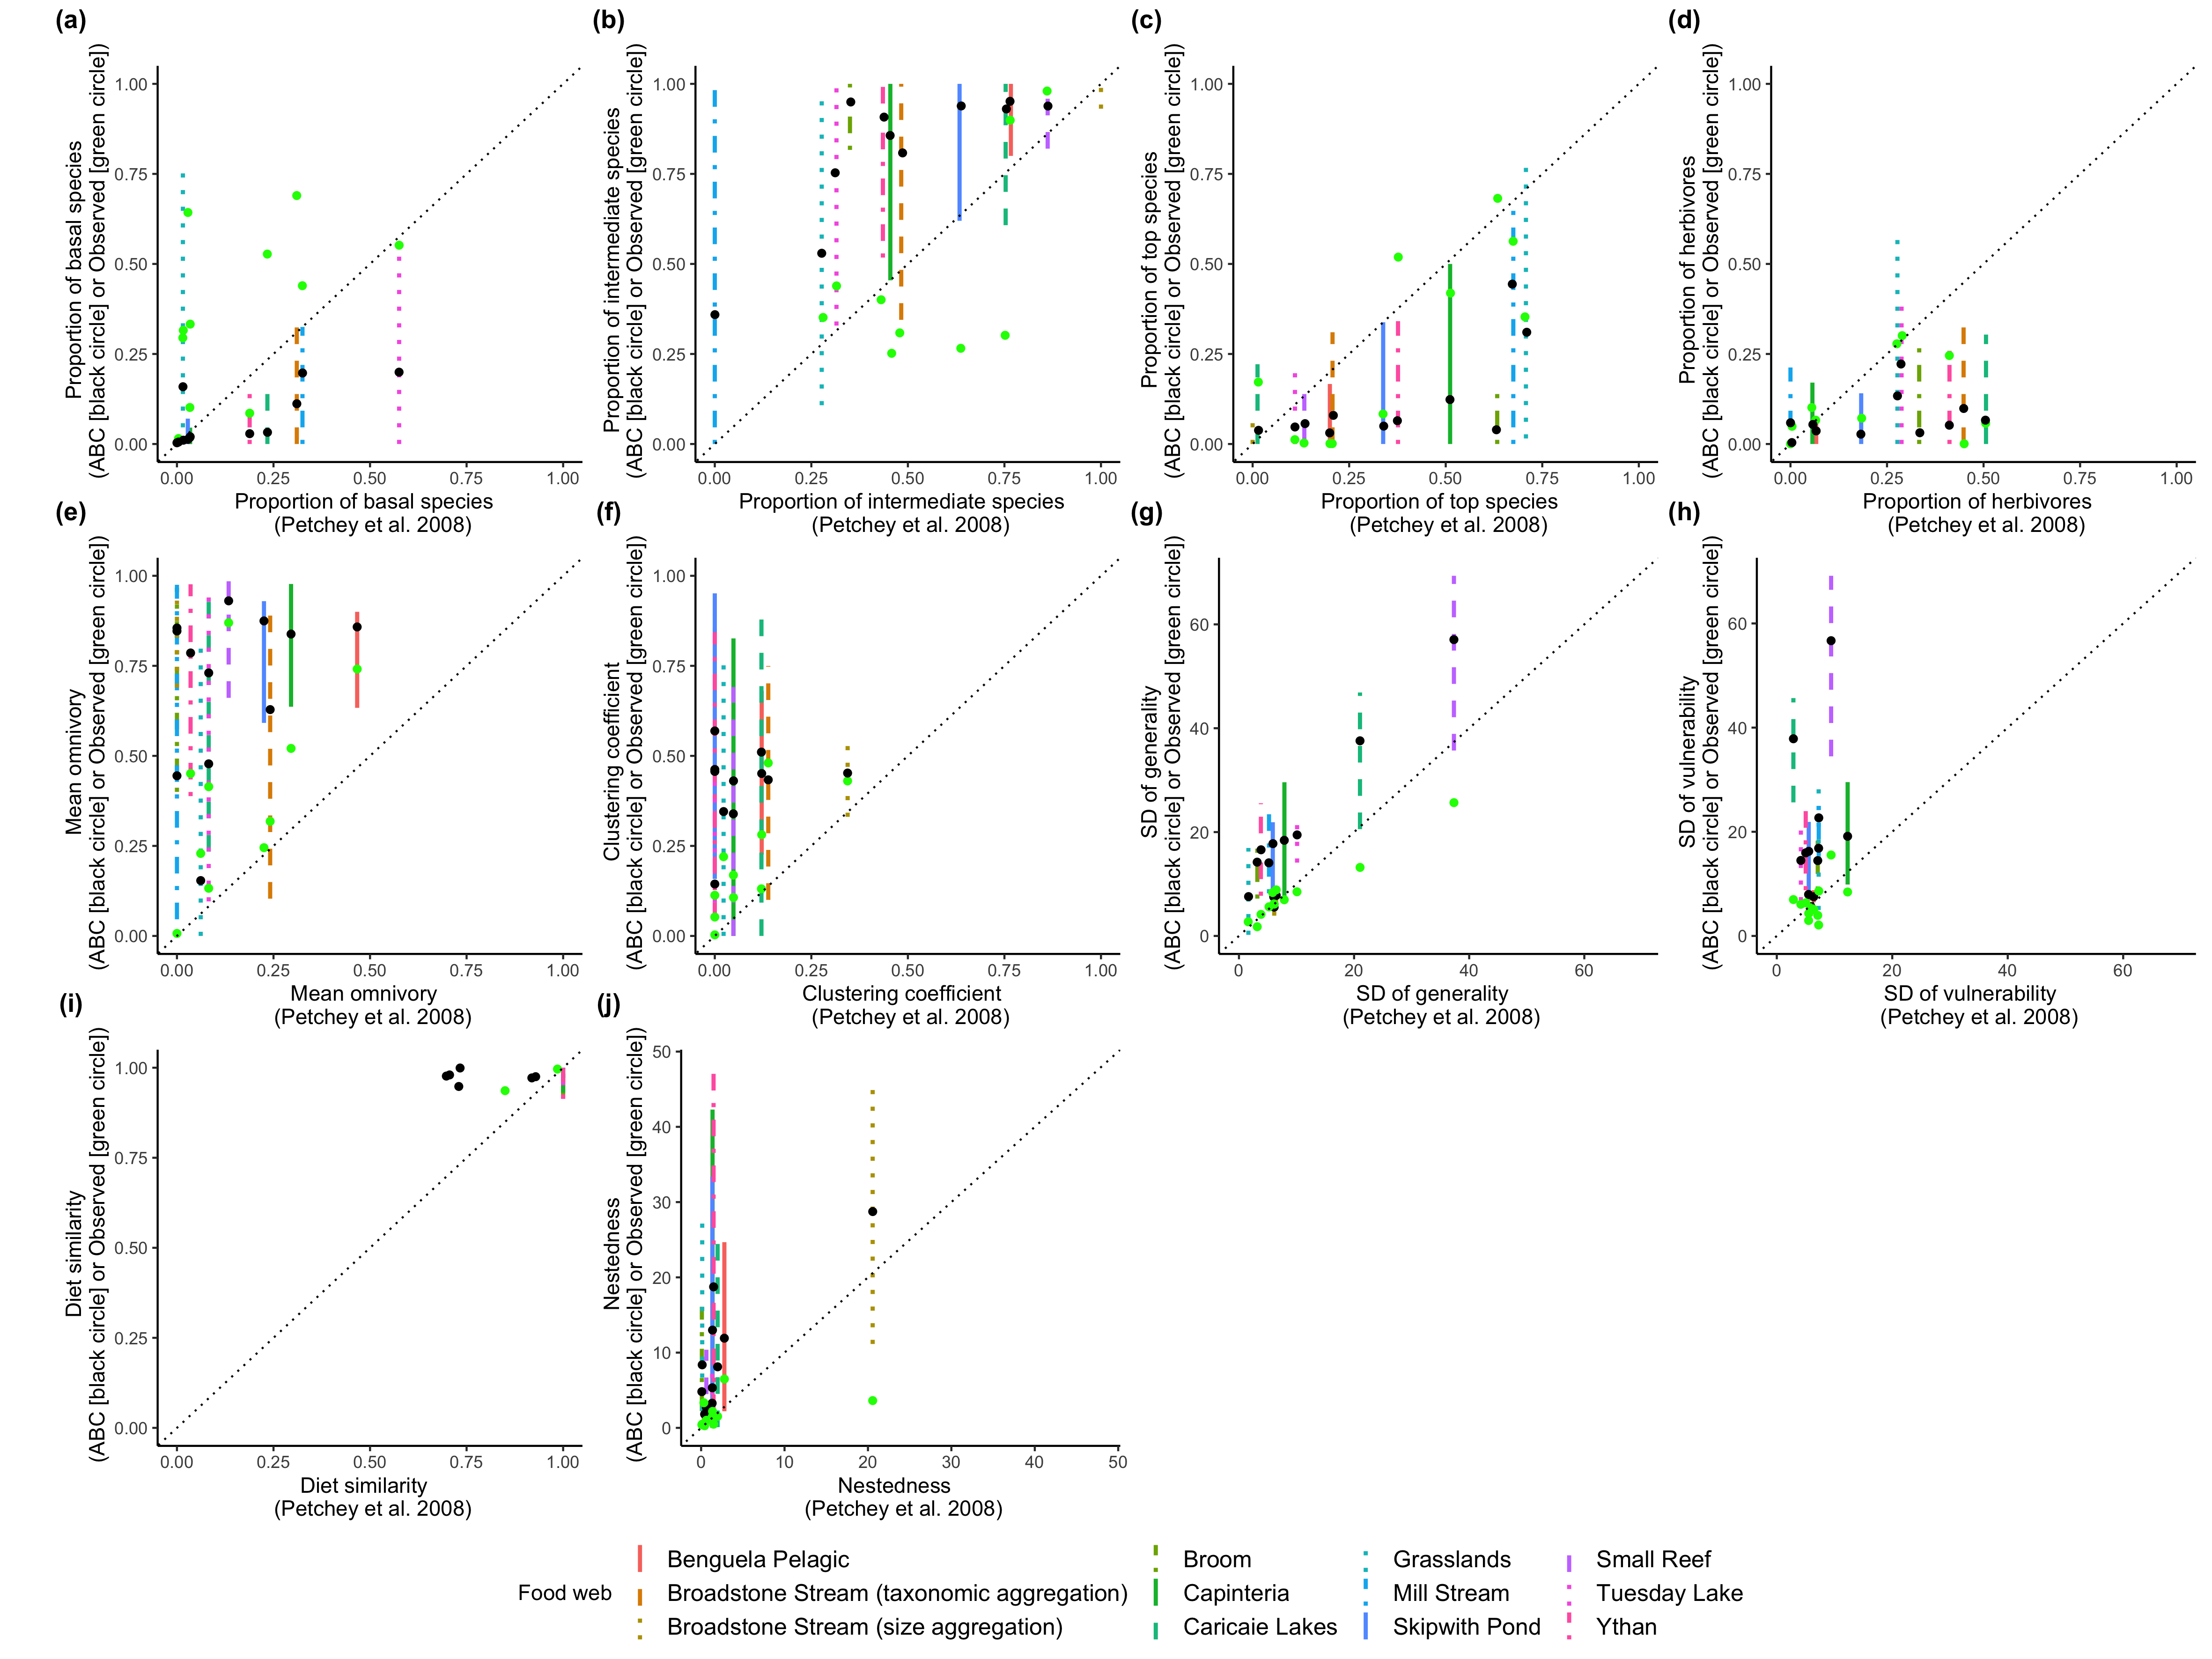
\includegraphics[width=500px]{../results/misc/r_properties_ABC_vs_petchey_TSS_lower_a} 

}

\caption{\label{fig:fig_r4p5} Structural properties of predicted food webs with 95\% prediction interval parameterised using the ABC method plotted against the point estimates from Petchey et al. (2008). The black filled circles correspond to the mean, and green filled circles correspond to the properties of the observed food webs. The dashed black lines are the 1:1 relationships for reference.}\label{fig:unnamed-chunk-8}
\end{figure}

The real values of the proportion of intermediate species, mean
omnivory, clustering coefficient, sd of generality, sd of vulnerability
and nestedness, were mostly within the lower range of the predicted 95\%
interval. The proportion of basal species, proportion of top species,
proportion of herbivores were underestimated in comparison to the real
values for most of the food webs.

The ADBM, when parameterised with the ABC, generally better predicted
the structural food web properties, such as proportion of basal species
when the true skill statistics was higher (Fig. \ref{fig:fig_r5}(a))
across the 12 food webs. However, the ABC parameterised ADBM less
accurately predicted food web properties on average than in the PBRW
study (Fig. \ref{fig:fig_r5}(b)).

\begin{figure}

{\centering 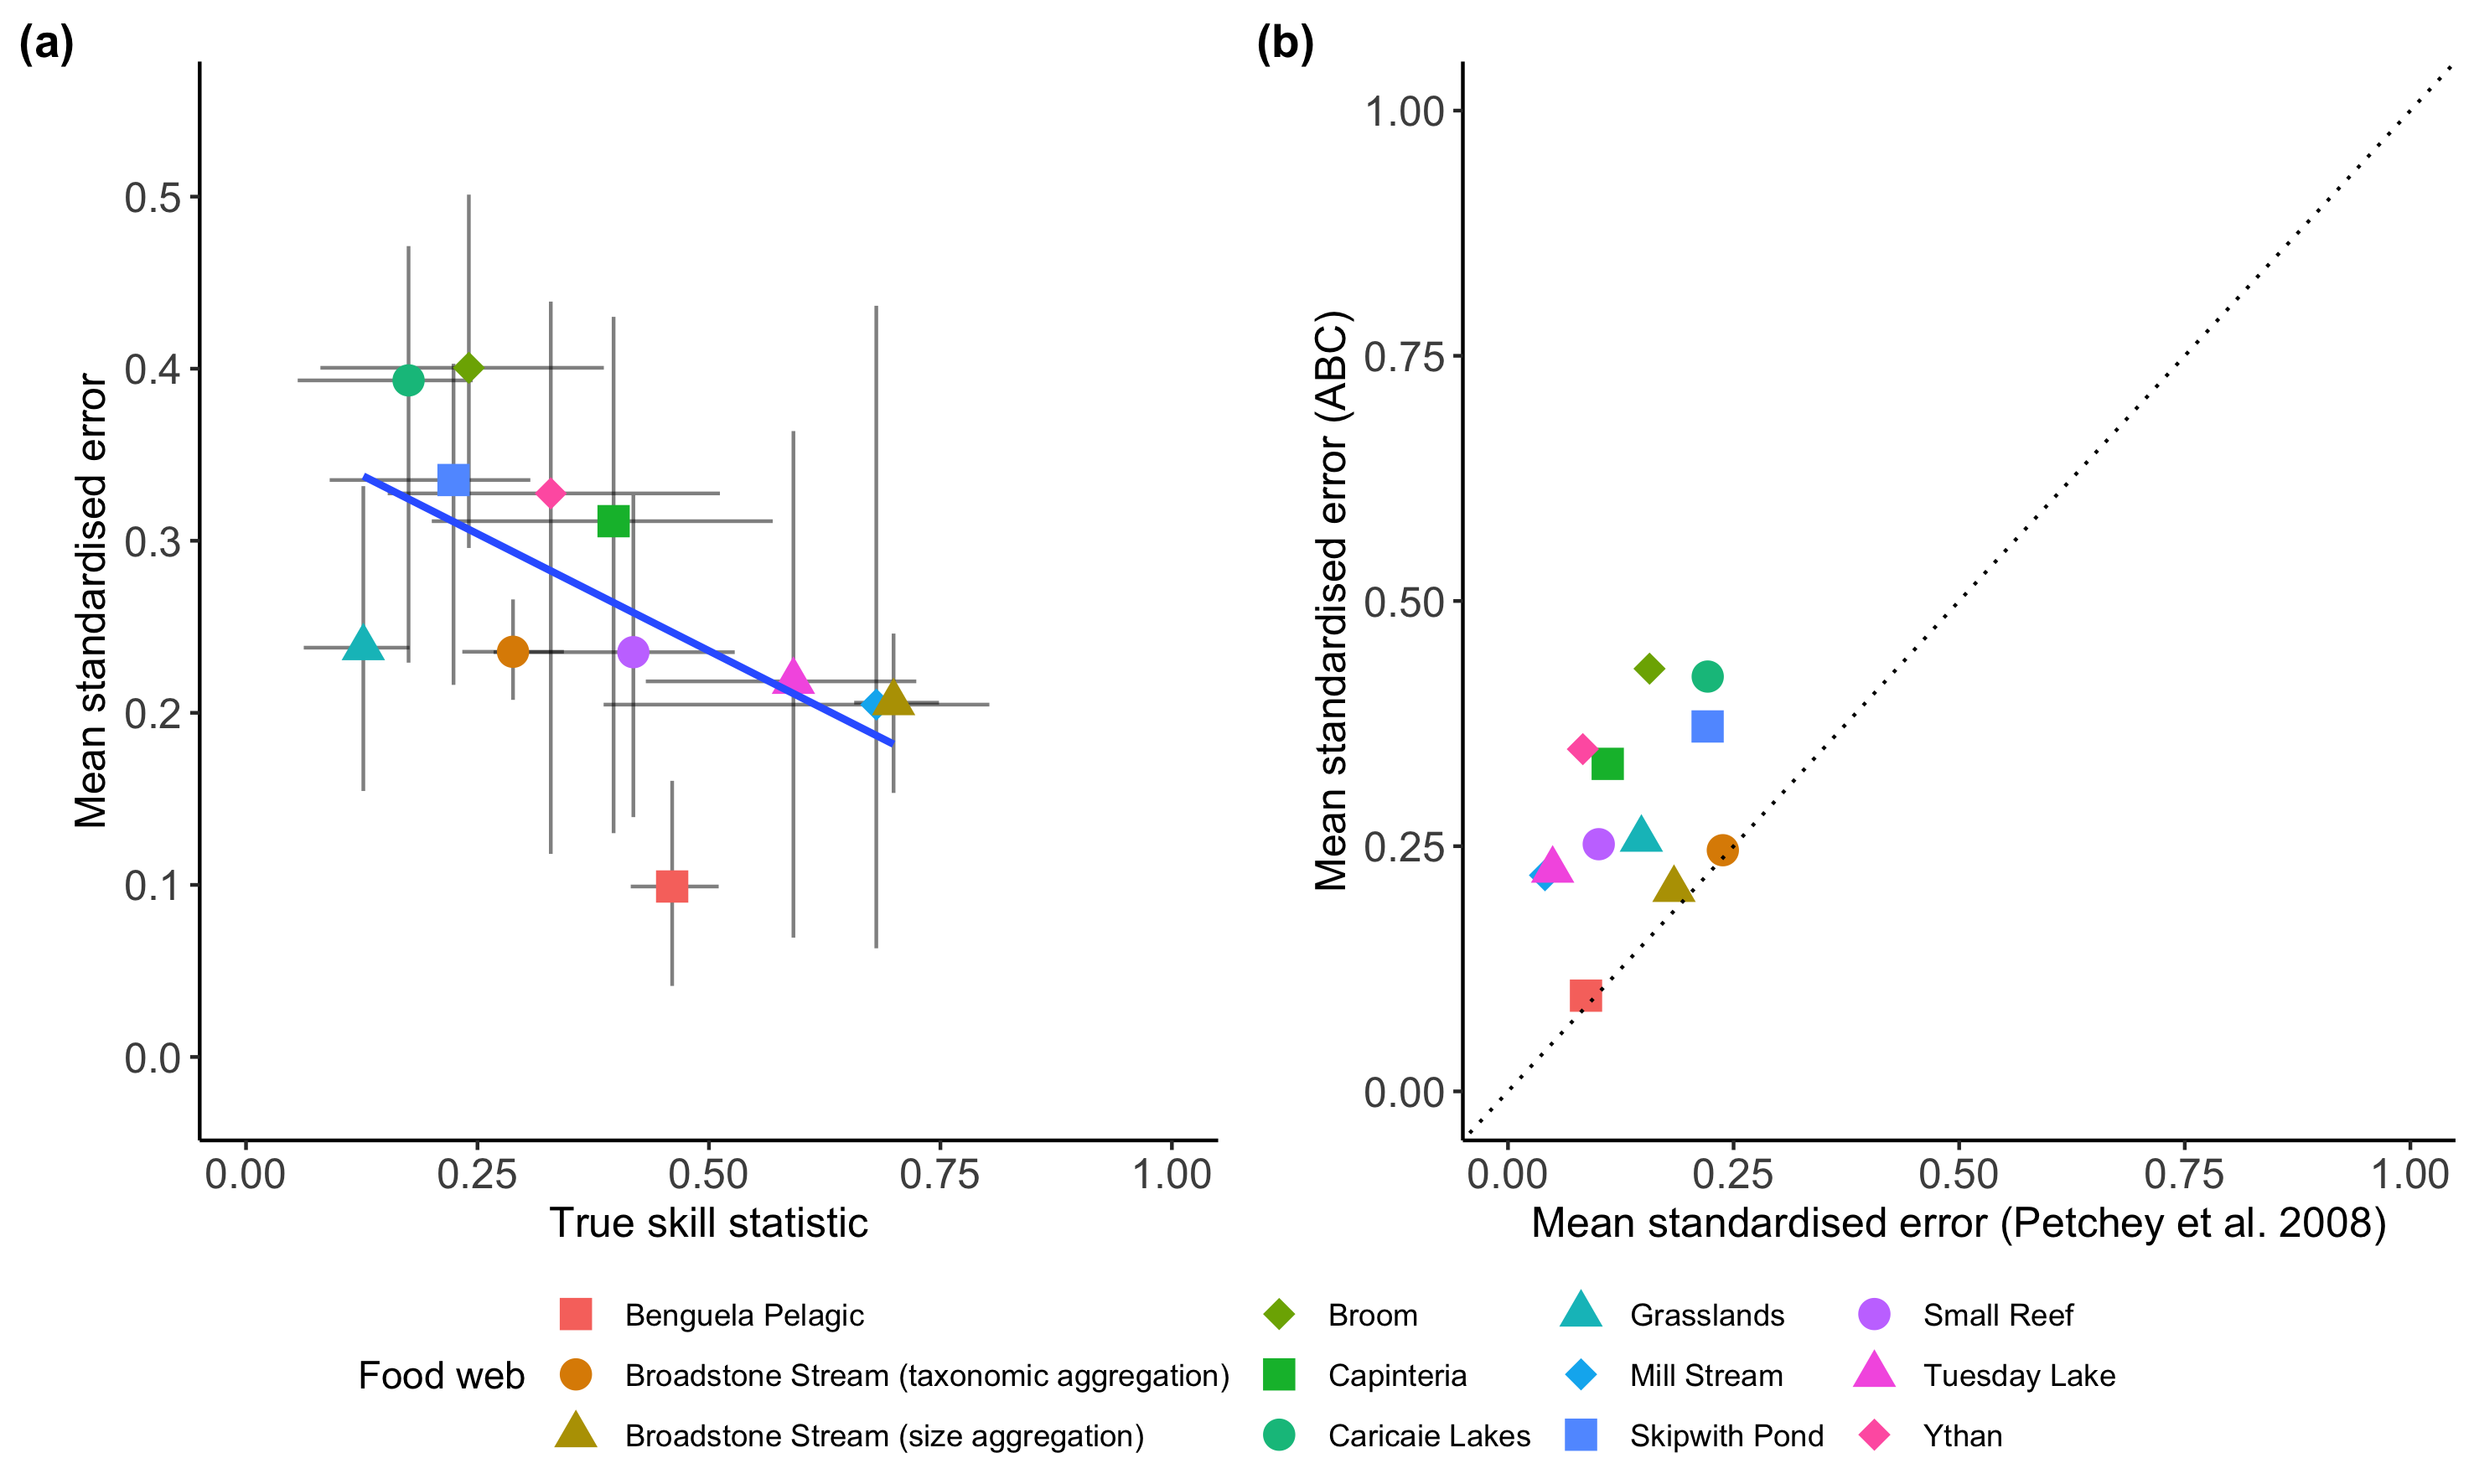
\includegraphics[width=400px]{fig/fig7} 

}

\caption{\label{fig:fig_r5} (a) The mean standardised error of the food web properties predicted from the ADBM parameterised using rejection ABC plotted against the mean true skill statistic for each food webs. The vertical and horizontal bars correspond to 95\% prediction intervals of the standardised error and true skill statistic respectively. Solid blue line is linear regression through the means (t = -2.335, df = 10, P = 0.041). (b) The mean standardised error computed from the ABC method plotted against the mean standardised error from Petchey et al. (2008). The dashed line is the 1:1 relationship for reference.}\label{fig:unnamed-chunk-9}
\end{figure}

Within each food web, we found various relationships between the
standardised error and true skill statistic (SI Figs S30 and S31). E.g.
For Skipwith Pond food web (SI Fig. S30(h)), high values of TSS were
associated with high error, whereas the opposite was true for other food
webs, such as Broadstone Stream (SI Fig. S30(b, l)). The other food webs
showed more complex relationships. The shapes of the point scatters in
SI Figs S30-31 are caused by the structural constraints of the ADBM
(e.g.~it can only predict contiguous diets) interacting with the TSS and
the connectance of the observed food web. These features prevent, for
example, a predicted food web with very high connectance having high
TSS. Similarly, a predicted food web with connectance equal to that of
the highest TSS prediction tends to have low TSS.

\hypertarget{discussion}{%
\section{Discussion}\label{discussion}}

The ABC parameterisation method employed here improves on the basic
parameterisation methods applied in Petchey et al. (2008) (PBRW). The
ABC method provides uncertainty in parameter estimates, and thereby a
range of predicted food webs (Fig. \ref{fig:fig_r2}(c-f)). It also
allowed us to estimate parameters that were fixed by the PBRW study, and
thereby also predicts connectance (Fig. \ref{fig:fig_r2}(b)). Including
uncertainty and predicting connectance are significant advances in ADBM.
They allow predictions in changes of food web structure caused by
environmental changes that include uncertainty in the predicted food web
structure and including uncertainty in such predictions is critical
(Petchey et al. 2015; Cressie et al. 2009; Lindegren et al. 2010). A
future development will be to partition the contribution of different
sources of uncertainty such as incomplete sampling and model
deficiencies to make improvements in the model with the aim of reducing
uncertainty. Future research should investigate the functional and
dynamical significance of the uncertainty in the predicted food web
structure. Below we discuss some of the results of our study, and expand
on these opportunities and priorities for future research.

In all cases, the predicted connectance was greater than the observed
connectance (Fig. \ref{fig:fig_r2}(b)). Why did this occur? Firstly, it
is important to recognise that the ADBM (when using only body size as a
trait) can only predict diets that are contiguous with respect to the
size of prey. I.e. it cannot predict that a predator will consume prey
of size 1 and 3, and not prey of size 2. Such patterns can however be
predicted if a trait in addition to size and which is not perfectly
correlated with size, influences foraging parameters (Petchey et al.
2008; Allesina, Alonso, and Pascual 2008; Stouffer, Camacho, and Amaral
2006). Secondly, it is important to note that the observed diets were
not contiguous when prey are ordered by their size. The estimation
process will result in a greater number of predicted links than observed
given these features, and the model attempts to maximise the coincidence
of predicted and observed link presence and absence (i.e.~the true skill
statistic).

These findings raise the question as to whether the model or the
observed data is incorrect. We expect that some of the links that do in
reality occur are not present in the empirical datasets. This could be
caused by low empirical sampling effort or rare prey-predator
interactions even when sampling is extensive. In this case, a false
positive may actually be a correctly predicted link. More intensive and
more complete sampling of links in food webs has been recognised as
important, due to the potential that a low sampling effort will
influence the perceived food web structure (Martinez et al. 1999).

We expect there are also cases of real false positives, where the model
predicts a feeding link despite no possibility that such a link could
occur in reality. This may be the case when a trait other than, or in
addition to, prey size is influential. For example, a particular prey
species may have a defensive trait that means it takes longer to consume
it than an undefended prey of the same size. Incorporating traits other
than body size in the ADBM would allow for discontiguous diets along the
size axis. It is also possible that better estimates of parameters that
could result from acquisition of new empirical data, could cause lower
estimated values of connectance. Furthermore, the ADBM's current form is
a biology-only model; it does not include an observation process,
although this could be included. The model would then be able to predict
the absence of a link due to incomplete observations.

It would be interesting to take a very well sampled food web (real or
simulated) and remove links at random to create a less well sampled
version, and to test if the very well sampled version can be predicted
from the less well sampled version (with ABC parameter estimation). If
it could, then there is potential to compensate for under-sampling with
an appropriate food web model and estimation procedure.

The ABC parameterisation resulted in a lower prediction accuracy of
structural features of the food webs (Fig. \ref{fig:fig_r5} (b)) due to
the overestimation of connectance. This was confirmed by principal
component analysis of variation in the food web structural properties
which revealed a first PC axis representing on average 62\% of the
overall variance, and this first axis was highly correlated with
connectance, with an average Spearman correlation of 0.87 (see SI S8 for
details). Furthermore, there was a strong positive relationship between
the mean standardised error in structural properties of the food webs
and mean standardised error in connectance of the food webs (SI Fig.
S32).

Our parameterisation approach was to maximise the true skill statistic
(the coincidence of predicted and observed link presences, and the
coincidence of predicted and observed link absences). The TSS assigns
equal importance to the collection of presence and absence of observed
links with the weight of an observed single presence or absence link
being dependent on the connectance of the food web. If the connectance
is less than 0.5, the TSS assigns more weight to a presence of link than
to an absence of a link and vice versa.

Because the connectance of the observed food webs is less than 0.5
(Table 1), the TSS implicitly assigned more weight to a presence of link
than to an absence of link. This upweighting of link presences seems
appropriate since observing a feeding interaction is unambiguous,
whereas not observing one may be caused by various processes. That is to
say, the observation of a single feeding interaction is sufficient to
record the presence of a link, whereas this is not true for the absence
of links: one observation of a predator not consuming a prey does not
mean that it will never do so.

To improve our estimation procedure we could quantify the uncertainty in
the recorded absence of links and include this uncertainty in the
parameterisation method. Weight/importance could be assigned to true
positives, true negatives, false positives and false negatives
calculated from empirical studies which may be specific to that food
web. Alternatively, an observation process could be added to the model,
such that the biological part of the model can predict that a feeding
link is possible, but then the observation process in the model leads to
that link not being predicted.

In the PBRW study, the parameter \(b\) played a major role in
maintaining the maximum predictive power of the ADBM. Indeed, they found
that estimating \(b\) only, and not estimating either \(a_i\) or \(a_j\)
slightly decreased model performance, and that estimating only \(b\) and
\(a_j\) did not decrease model performance relative to when all three
parameters were estimated.

We found that the posterior distribution of the parameter \(b\) was the
most constrained of all the parameters (Fig. \ref{fig:fig_r3}).
Parameter \(b\) defines the range of prey body size which has a finite
handling time, and the prey size with the highest energetic
profitability. As the parameter \(b\) relates to the prey-predator body
size ratio, the constrained posterior of \(b\) (Fig.
\ref{fig:fig_r3}(d)) indicates the importance of the ratio of body size
of prey and predator in determining the food web structure with the
ADBM.

The marginal posterior of parameter \(a\) was right-skewed (Fig.
\ref{fig:fig_r3}(c)). This may be because the ABC parameterisation
overestimates the connectance, which means that lower values of \(a\)
are preferred over higher values of \(a\) (a lower value of \(a\) leads
to a lower space clearance/attack rate, and a lower space clearance rate
results in a higher connectance).

Information about who eats whom can be collected from multiple sources,
such as gut contents of organisms, stable isotope composition of
tissues, and experimentation (Peralta-Maraver, López-Rodríguez, and de
Figueroa 2017; Layman et al. 2007; Warren 1989). Moreover,
experimentation provides independent estimates of allometric foraging
parameters, such as \(b\), \(a_i\), and \(a_j\) (Rall et al. 2012).
Diverse data could be used to parameterise the ADBM's predictions to
test how uncertainty in the different datasets influences the ADBM's
predictions using ABC. Appropriate summary statistics in the ABC method
could be used to address such challenges. We could use, as an example,
the approximate trophic position inferred from stable isotope ratio data
from an individual tissue and gut content data of a predator
simultaneously to parameterise the ADBM. The trophic position and the
gut content information would be the summary statistics in this example.
A further question that could be addressed in future studies is how the
quantity of data affects the ADBM's predictions. The outcome of such a
study could help food web researchers decide on how much data from a
specific source is needed to predict the food web structure, and help
further optimise the deployment of limited sampling resources.

When only partial food web data is available (Patonai and Jord'an 2017),
the summary statistics in ABC can be used to infer these food web
structures from the ADBM. It would be possible to use gut content data
of only some of the species in a food web to parameterise the ADBM and
predict the food web structure. Summary statistics opens up a broad
spectrum of possibilities in parameterising food web models. There are
multiple empirical and theoretical studies on a range of different food
web properties of food webs across different ecosystems (Williams and
Martinez 2000; Goldwasser and Roughgarden 1993; Martinez 1991). These
can conceivably be used in parameterising food web models using ABC to
constrain the model predictions.

\hypertarget{acknowledgements}{%
\section{Acknowledgements}\label{acknowledgements}}

This work was supported by the University Research Priority Program
Global Change and Biodiversity (Grant number: U-704-04-11) of the
University of Zurich. We thank the Petchey group members for their
valuable suggestions in the manuscript. We thank Debra Zuppinger-Dingley
for proofreading the manuscript.

\hypertarget{author-contributions}{%
\section{Author contributions}\label{author-contributions}}

Anubhav Gupta: Conceptualization (equal), data curation (lead), formal
analysis (lead), investigation (lead), methodology (lead), project
administration (lead), software (lead), validation (lead), visualisation
(lead), writing -- original draft preparation (lead), writing - review
and editing (equal). Reinhard Furrer: Methodology (supporting). Owen L.
Petchey: Conceptualization (equal), funding acquisition (lead),
methodology (supporting), resources (lead), supervision (lead), writing
-- original draft preparation (supporting), writing - review and editing
(equal).

\hypertarget{data-accessibility-statement}{%
\section{Data Accessibility
Statement}\label{data-accessibility-statement}}

All the data used in this study was collected in other studies and is
openly available. We list those studies and the open access source in
Table \ref{fig:tab_1}. The code used for data curation is available in
the repository \url{https://github.com/anubhav3/C1_data}. The code used
for fitting the ADBM using the point parameterisation method in Petchey
et al. (2008) is available in the repository
\url{https://github.com/anubhav3/C1_ADBM_2008_fitting}. The complete
code used in the analysis is available in the repository
\url{https://github.com/anubhav3/C1_method_v2}.

\hypertarget{references}{%
\section*{References}\label{references}}
\addcontentsline{toc}{section}{References}

\hypertarget{refs}{}
\begin{CSLReferences}{1}{0}
\leavevmode\hypertarget{ref-allesina2008}{}%
Allesina, Stefano, David Alonso, and Mercedes Pascual. 2008. {``A
General Model for Food Web Structure.''} \emph{Science} 320 (5876):
658--61. \url{https://doi.org/10.1126/science.1156269}.

\leavevmode\hypertarget{ref-bakerFishGutContent2014}{}%
Baker, Ronald, Amanda Buckland, and Marcus Sheaves. 2014. {``Fish Gut
Content Analysis: Robust Measures of Diet Composition.''} \emph{Fish and
Fisheries} 15 (1): 170--77. \url{https://doi.org/10.1111/faf.12026}.

\leavevmode\hypertarget{ref-beckermanForagingBiologyPredicts2006}{}%
Beckerman, A. P., O. L. Petchey, and P. H. Warren. 2006. {``Foraging
Biology Predicts Food Web Complexity.''} \emph{Proceedings of the
National Academy of Sciences} 103 (37): 13745--49.
\url{https://doi.org/10.1073/pnas.0603039103}.

\leavevmode\hypertarget{ref-bergaminoFoodWebStructure2011}{}%
Bergamino, Leandro, Diego Lercari, and Omar Defeo. 2011. {``Food Web
Structure of Sandy Beaches: {Temporal} and Spatial Variation Using
Stable Isotope Analysis.''} \emph{Estuarine, Coastal and Shelf Science}
91 (4): 536--43. \url{https://doi.org/10.1016/j.ecss.2010.12.007}.

\leavevmode\hypertarget{ref-broseBodySizesConsumers2005}{}%
Brose, Ulrich, Lara Cushing, Eric L. Berlow, Tomas Jonsson, Carolin
Banasek-Richter, Louis-Felix Bersier, Julia L. Blanchard, et al. 2005.
{``Body {Sizes} of {Consumers} and {Their Resources}.''} \emph{Ecology}
86 (9): 2545--45. \url{https://doi.org/10.1890/05-0379}.

\leavevmode\hypertarget{ref-carpenterEcologicalFuturesBuilding2016}{}%
Carpenter, Stephen R. 2016. {``Ecological Futures: Building an Ecology
of the Long Now.''} \emph{Ecology}, October, 2069--83.
\url{https://doi.org/10.1890/0012-9658(2002)083\%5B2069:EFBAEO\%5D2.0.CO;2@10.1002/(ISSN)1939-9170.MacArthurAward}.

\leavevmode\hypertarget{ref-cattinPhylogeneticConstraintsAdaptation2004}{}%
Cattin, Marie-France, Louis-F'elix Bersier, Carolin Banašek-Richter,
Richard Baltensperger, and Jean-Pierre Gabriel. 2004. {``Phylogenetic
Constraints and Adaptation Explain Food-Web Structure.''} \emph{Nature}
427 (6977, 6977): 835--39. \url{https://doi.org/10.1038/nature02327}.

\leavevmode\hypertarget{ref-cirtwill2018feeding}{}%
Cirtwill, Alyssa R, and Anna Eklöf. 2018. {``Feeding Environment and
Other Traits Shape Species' Roles in Marine Food Webs.''} \emph{Ecology
Letters} 21 (6): 875--84.

\leavevmode\hypertarget{ref-cohenStochasticTheoryCommunity1985}{}%
Cohen, Joel E., C. M. Newman, and John Hyslop Steele. 1985. {``A
Stochastic Theory of Community Food Webs {I}. {Models} and Aggregated
Data.''} \emph{Proceedings of the Royal Society of London. Series B.
Biological Sciences} 224 (1237): 421--48.
\url{https://doi.org/10.1098/rspb.1985.0042}.

\leavevmode\hypertarget{ref-crawfordApplicationsStableIsotope2008}{}%
Crawford, Kerry, Robbie A. Mcdonald, and Stuart Bearhop. 2008.
{``Applications of Stable Isotope Techniques to the Ecology of
Mammals.''} \emph{Mammal Review} 38 (1): 87--107.
\url{https://doi.org/10.1111/j.1365-2907.2008.00120.x}.

\leavevmode\hypertarget{ref-cressieAccountingUncertaintyEcological2009}{}%
Cressie, Noel, Catherine A. Calder, James S. Clark, Jay M. Ver Hoef, and
Christopher K. Wikle. 2009. {``Accounting for Uncertainty in Ecological
Analysis: The Strengths and Limitations of Hierarchical Statistical
Modeling.''} \emph{Ecological Applications} 19 (3): 553--70.
\url{https://doi.org/10.1890/07-0744.1}.

\leavevmode\hypertarget{ref-dawahStructureParasitoidCommunities1995}{}%
Dawah, Hassan Ali, Bradford A. Hawkins, and Michael F. Claridge. 1995.
{``Structure of the {Parasitoid Communities} of {Grass}-{Feeding Chalcid
Wasps}.''} \emph{The Journal of Animal Ecology} 64 (6): 708.
\url{https://doi.org/10.2307/5850}.

\leavevmode\hypertarget{ref-dunneNetworkStructureBiodiversity}{}%
Dunne, Jennifer A., Richard J. Williams, and Neo D. Martinez. 2002.
{``Network Structure and Biodiversity Loss in Food Webs: Robustness
Increases with Connectance.''} \emph{Ecology Letters} 5 (4): 558--67.

\leavevmode\hypertarget{ref-emmersonPredatorPreyBody2004}{}%
Emmerson, Mark C., and Dave Raffaelli. 2004. {``Predator--Prey Body
Size, Interaction Strength and the Stability of a Real Food Web.''}
\emph{Journal of Animal Ecology} 73 (3): 399--409.
\url{https://doi.org/10.1111/j.0021-8790.2004.00818.x}.

\leavevmode\hypertarget{ref-goldwasserConstructionAnalysisLarge1993}{}%
Goldwasser, Lloyd, and Jonathan Roughgarden. 1993. {``Construction and
{Analysis} of a {Large Caribbean Food Web}: {Ecological Archives
E074}-001.''} \emph{Ecology} 74 (4): 1216--33.
\url{https://doi.org/10.2307/1940492}.

\leavevmode\hypertarget{ref-gravelInferringFoodWeb2013}{}%
Gravel, Dominique, Timoth'ee Poisot, Camille Albouy, Laure Velez, and
David Mouillot. 2013. {``Inferring Food Web Structure from Predator-Prey
Body Size Relationships.''} Edited by Robert Freckleton. \emph{Methods
in Ecology and Evolution} 4 (11): 1083--90.
\url{https://doi.org/10.1111/2041-210X.12103}.

\leavevmode\hypertarget{ref-harper-smithCOMMUNICATINGECOLOGYFOOD2005}{}%
Harper-Smith, Sarah, Eric L. Berlow, Roland A. Knapp, Richard J.
Williams, and Neo D. Martinez. 2005. {``{COMMUNICATING ECOLOGY THROUGH
FOOD WEBS}: {VISUALIZING AND QUANTIFYING THE EFFECTS OF STOCKING ALPINE
LAKES WITH TROUT}.''} In \emph{Dynamic {Food Webs}}, 407--23.
{Elsevier}. \url{https://doi.org/10.1016/B978-012088458-2/50038-2}.

\leavevmode\hypertarget{ref-hattabForecastingFinescaleChanges2016}{}%
Hattab, Tarek, Fabien Leprieur, Frida Ben Rais Lasram, Dominique Gravel,
François Le Loc'h, and Camille Albouy. 2016. {``Forecasting Fine-Scale
Changes in the Food-Web Structure of Coastal Marine Communities Under
Climate Change.''} \emph{Ecography} 39 (12): 1227--37.
\url{https://doi.org/10.1111/ecog.01937}.

\leavevmode\hypertarget{ref-hechinger2011food}{}%
Hechinger, Ryan F, Kevin D Lafferty, John P McLaughlin, Brian L
Fredensborg, Todd C Huspeni, Julio Lorda, Parwant K Sandhu, et al. 2011.
{``Food Webs Including Parasites, Biomass, Body Sizes, and Life Stages
for Three California/Baja California Estuaries: Ecological Archives
E092-066.''} \emph{Ecology} 92 (3): 791--91.

\leavevmode\hypertarget{ref-hobsonUsingStableIsotopes1994}{}%
Hobson, Keith A., John F. Piatt, and Jay Pitocchelli. 1994. {``Using
{Stable Isotopes} to {Determine Seabird Trophic Relationships}.''}
\emph{Journal of Animal Ecology} 63 (4): 786--98.
\url{https://doi.org/10.2307/5256}.

\leavevmode\hypertarget{ref-hudsonCheddarAnalysisVisualisation2013}{}%
Hudson, Lawrence N., Rob Emerson, Gareth B. Jenkins, Katrin Layer, Mark
E. Ledger, Doris E. Pichler, Murray S. A. Thompson, Eoin J. O'Gorman,
Guy Woodward, and Daniel C. Reuman. 2013. {``Cheddar: Analysis and
Visualisation of Ecological Communities in {R}.''} \emph{Methods in
Ecology and Evolution} 4 (1): 99--104.
\url{https://doi.org/10.1111/2041-210X.12005}.

\leavevmode\hypertarget{ref-ibanezOptimizingSizeThresholds2012}{}%
Ibanez, S'ebastien. 2012. {``Optimizing Size Thresholds in a
Plant--Pollinator Interaction Web: Towards a Mechanistic Understanding
of Ecological Networks.''} \emph{Oecologia} 170 (1): 233--42.
\url{https://doi.org/10.1007/s00442-012-2290-3}.

\leavevmode\hypertarget{ref-jabotInferringParametersNeutral2009}{}%
Jabot, Franck, and J'erôme Chave. 2009. {``Inferring the Parameters of
the Neutral Theory of Biodiversity Using Phylogenetic Information and
Implications for Tropical Forests.''} \emph{Ecology Letters} 12 (3):
239--48. \url{https://doi.org/10.1111/j.1461-0248.2008.01280.x}.

\leavevmode\hypertarget{ref-jonssonFoodWebsBody2005}{}%
Jonsson, Tomas, Joel E. Cohen, and Stephen R. Carpenter. 2005. {``Food
{Webs}, {Body Size}, and {Species Abundance} in {Ecological Community
Description}.''} In \emph{Advances in {Ecological Research}}, 36:1--84.
{Elsevier}. \url{https://doi.org/10.1016/S0065-2504(05)36001-6}.

\leavevmode\hypertarget{ref-jordanSensitivityFoodWeb2009}{}%
Jord'an, Ferenc, and Györgyi Osv'ath. 2009. {``The Sensitivity of Food
Web Topology to Temporal Data Aggregation.''} \emph{Ecological
Modelling} 220 (22): 3141--46.
\url{https://doi.org/10.1016/j.ecolmodel.2009.05.002}.

\leavevmode\hypertarget{ref-knightTrophicCascadesEcosystems2005}{}%
Knight, Tiffany M., Michael W. McCoy, Jonathan M. Chase, Krista A.
McCoy, and Robert D. Holt. 2005. {``Trophic Cascades Across
Ecosystems.''} \emph{Nature} 437 (7060): 880--83.
\url{https://doi.org/10.1038/nature03962}.

\leavevmode\hypertarget{ref-krauseCompartmentsRevealedFoodweb2003}{}%
Krause, Ann E., Kenneth A. Frank, Doran M. Mason, Robert E. Ulanowicz,
and William W. Taylor. 2003. {``Compartments Revealed in Food-Web
Structure.''} \emph{Nature} 426 (6964): 282--85.
\url{https://doi.org/10.1038/nature02115}.

\leavevmode\hypertarget{ref-laffertyParasitesDominateFood2006}{}%
Lafferty, K. D., A. P. Dobson, and A. M. Kuris. 2006. {``Parasites
Dominate Food Web Links.''} \emph{Proceedings of the National Academy of
Sciences} 103 (30): 11211--16.
\url{https://doi.org/10.1073/pnas.0604755103}.

\leavevmode\hypertarget{ref-laymanCanStableIsotope2007}{}%
Layman, Craig A., D. Albrey Arrington, Carmen G. Montaña, and David M.
Post. 2007. {``Can {Stable Isotope Ratios Provide} for {Community}-{Wide
Measures} of {Trophic Structure}?''} \emph{Ecology} 88 (1): 42--48.
\url{https://doi.org/10.1890/0012-9658(2007)88\%5B42:CSIRPF\%5D2.0.CO;2}.

\leavevmode\hypertarget{ref-lindegrenEcologicalForecastingClimate2010}{}%
Lindegren, Martin, Christian Möllmann, Anders Nielsen, Keith Brander,
Brian R. MacKenzie, and Nils Chr. Stenseth. 2010. {``Ecological
Forecasting Under Climate Change: The Case of {Baltic} Cod.''}
\emph{Proceedings of the Royal Society B: Biological Sciences} 277
(1691): 2121--30. \url{https://doi.org/10.1098/rspb.2010.0353}.

\leavevmode\hypertarget{ref-lurgiClimateChangeImpacts2012}{}%
Lurgi, Miguel, Bernat C. L'opez, and Jos'e M. Montoya. 2012. {``Climate
Change Impacts on Body Size and Food Web Structure on Mountain
Ecosystems.''} \emph{Philosophical Transactions of the Royal Society B:
Biological Sciences} 367 (1605): 3050--57.
\url{https://doi.org/10.1098/rstb.2012.0239}.

\leavevmode\hypertarget{ref-macarthurOptimalUsePatchy1966}{}%
MacArthur, Robert H., and Eric R. Pianka. 1966. {``On {Optimal Use} of a
{Patchy Environment}.''} \emph{The American Naturalist} 100 (916):
603--9.

\leavevmode\hypertarget{ref-martinezArtifactsAttributesEffects1991}{}%
Martinez, Neo D. 1991. {``Artifacts or {Attributes}? {Effects} of
{Resolution} on the {Little Rock Lake Food Web}.''} \emph{Ecological
Monographs} 61 (4): 367--92. \url{https://doi.org/10.2307/2937047}.

\leavevmode\hypertarget{ref-martinezEffectsSamplingEffort1999}{}%
Martinez, Neo D., Bradford A. Hawkins, Hassan Ali Dawah, and Brian P.
Feifarek. 1999. {``Effects of {Sampling Effort} on {Characterization} of
{Food}-{Web Structure}.''} \emph{Ecology} 80 (3): 1044--55.
\url{https://doi.org/10.1890/0012-9658(1999)080\%5B1044:EOSEOC\%5D2.0.CO;2}.

\leavevmode\hypertarget{ref-mayWillLargeComplex1972}{}%
May, Robert M. 1972. {``Will a {Large Complex System} Be {Stable}?''}
\emph{Nature} 238 (5364): 413. \url{https://doi.org/10.1038/238413a0}.

\leavevmode\hypertarget{ref-memmottPredatorsParasitoidsPathogens2000}{}%
Memmott, J., N. D. Martinez, and J. E. Cohen. 2000. {``Predators,
Parasitoids and Pathogens: Species Richness, Trophic Generality and Body
Sizes in a Natural Food Web.''} \emph{Journal of Animal Ecology} 69 (1):
1--15. \url{https://doi.org/10.1046/j.1365-2656.2000.00367.x}.

\leavevmode\hypertarget{ref-morrisFoodWebStructure2015}{}%
Morris, Rebecca J., Frazer H. Sinclair, and Chris J. Burwell. 2015.
{``Food Web Structure Changes with Elevation but Not Rainforest
Stratum.''} \emph{Ecography} 38 (8): 792--802.
\url{https://doi.org/10.1111/ecog.01078}.

\leavevmode\hypertarget{ref-oconnorWarmingResourceAvailability2009}{}%
O'Connor, Mary I., Michael F. Piehler, Dina M. Leech, Andrea Anton, and
John F. Bruno. 2009. {``Warming and {Resource Availability Shift Food
Web Structure} and {Metabolism}.''} Edited by Michel Loreau. \emph{PLoS
Biology} 7 (8): e1000178.
\url{https://doi.org/10.1371/journal.pbio.1000178}.

\leavevmode\hypertarget{ref-opitz1996}{}%
Opitz, Silvia. 1996. {``Quantitative Models of Trophic Interactions in
Caribbean Coral Reefs.''}

\leavevmode\hypertarget{ref-patonaiAggregationIncompleteFood2017}{}%
Patonai, Katalin, and Ferenc Jord'an. 2017. {``Aggregation of Incomplete
Food Web Data May Help to Suggest Sampling Strategies.''}
\emph{Ecological Modelling} 352 (May): 77--89.
\url{https://doi.org/10.1016/j.ecolmodel.2017.02.024}.

\leavevmode\hypertarget{ref-peralta-maraverStructureDynamicsStability2016a}{}%
Peralta-Maraver, I., M. J. López-Rodríguez, and J. M. Tierno de
Figueroa. 2016. {``Structure, Dynamics and Stability of a
{Mediterranean} River Food Web.''} \emph{Marine and Freshwater Research}
68 (3): 484--95. \url{https://doi.org/10.1071/MF15154}.

\leavevmode\hypertarget{ref-peralta-maraverStructureDynamicsStability2017}{}%
---------. 2017. {``Structure, Dynamics and Stability of a
{Mediterranean} River Food Web.''} \emph{Marine and Freshwater Research}
68 (3): 484--95. \url{https://doi.org/10.1071/MF15154}.

\leavevmode\hypertarget{ref-petchey2008size}{}%
Petchey, Owen L., Andrew P. Beckerman, Jens O. Riede, and Philip H.
Warren. 2008. {``Size, Foraging, and Food Web Structure.''}
\emph{Proceedings of the National Academy of Sciences} 105: 4191--96.
\url{https://doi.org/10.1073/pnas.0710672105}.

\leavevmode\hypertarget{ref-petcheyEnvironmentalWarmingAlters1999}{}%
Petchey, Owen L., P. Timon McPhearson, Timothy M. Casey, and Peter J.
Morin. 1999. {``Environmental Warming Alters Food-Web Structure and
Ecosystem Function.''} \emph{Nature} 402 (6757): 69--72.
\url{https://doi.org/10.1038/47023}.

\leavevmode\hypertarget{ref-petcheyEcologicalForecastHorizon2015}{}%
Petchey, Owen L., Mikael Pontarp, Thomas M. Massie, Sonia K'efi, Arpat
Ozgul, Maja Weilenmann, Gian Marco Palamara, et al. 2015. {``The
Ecological Forecast Horizon, and Examples of Its Uses and
Determinants.''} \emph{Ecology Letters} 18 (7): 597--611.
\url{https://doi.org/10.1111/ele.12443}.

\leavevmode\hypertarget{ref-poisotWhenEcologicalNetwork2014}{}%
Poisot, Timoth'ee, and Dominique Gravel. 2014. {``When Is an Ecological
Network Complex? {Connectance} Drives Degree Distribution and Emerging
Network Properties.''} \emph{PeerJ} 2 (February): e251.
\url{https://doi.org/10.7717/peerj.251}.

\leavevmode\hypertarget{ref-poisotHowEcologicalNetworks2016}{}%
Poisot, Timoth'ee, and Daniel B. Stouffer. 2016. {``How Ecological
Networks Evolve.''} Preprint. {Ecology}.
\url{https://doi.org/10.1101/071993}.

\leavevmode\hypertarget{ref-rallUniversalTemperatureBodymass2012}{}%
Rall, B. C., U. Brose, M. Hartvig, G. Kalinkat, F. Schwarzmuller, O.
Vucic-Pestic, and O. L. Petchey. 2012. {``Universal Temperature and
Body-Mass Scaling of Feeding Rates.''} \emph{Philosophical Transactions
of the Royal Society B: Biological Sciences} 367 (1605): 2923--34.
\url{https://doi.org/10.1098/rstb.2012.0242}.

\leavevmode\hypertarget{ref-shrinerEvolutionIntrahostHiv2006}{}%
Shriner, Daniel, Yi Liu, David C. Nickle, and James I. Mullins. 2006.
{``Evolution of {Intrahost Hiv} - 1 {Genetic Diversity During Chronic
Infection}.''} \emph{Evolution} 60 (6): 1165--76.
\url{https://doi.org/10.1111/j.0014-3820.2006.tb01195.x}.

\leavevmode\hypertarget{ref-stoufferRobustMeasureFood2006}{}%
Stouffer, Daniel B., Juan Camacho, and Lu'ıs A. Nunes Amaral. 2006. {``A
Robust Measure of Food Web Intervality.''} \emph{Proceedings of the
National Academy of Sciences} 103 (50): 19015--20.
\url{https://doi.org/10.1073/pnas.0603844103}.

\leavevmode\hypertarget{ref-tamaddoni-nezhadConstructionValidationFood2013}{}%
Tamaddoni-Nezhad, Alireza, Ghazal Afroozi Milani, Alan Raybould, Stephen
Muggleton, and David A. Bohan. 2013. {``Construction and {Validation} of
{Food Webs Using Logic}-{Based Machine Learning} and {Text Mining}.''}
In \emph{Advances in {Ecological Research}}, 49:225--89. {Elsevier}.
\url{https://doi.org/10.1016/B978-0-12-420002-9.00004-4}.

\leavevmode\hypertarget{ref-toniApproximateBayesianComputation2009}{}%
Toni, Tina, David Welch, Natalja Strelkowa, Andreas Ipsen, and Michael
P. H. Stumpf. 2009. {``Approximate {Bayesian} Computation Scheme for
Parameter Inference and Model Selection in Dynamical Systems.''}
\emph{Journal of the Royal Society Interface} 6 (31): 187--202.
\url{https://doi.org/10.1098/rsif.2008.0172}.

\leavevmode\hypertarget{ref-tylianakisEffectsGlobalEnvironmental2014}{}%
Tylianakis, Jason M., and Amrei Binzer. 2014. {``Effects of Global
Environmental Changes on Parasitoid{}host Food Webs and Biological
Control.''} \emph{Biological Control} 75 (August): 77--86.
\url{https://doi.org/10.1016/j.biocontrol.2013.10.003}.

\leavevmode\hypertarget{ref-warrenSpatialTemporalVariation1989}{}%
Warren, Philip H. 1989. {``Spatial and {Temporal Variation} in the
{Structure} of a {Freshwater Food Web}.''} \emph{Oikos} 55 (3): 299.
\url{https://doi.org/10.2307/3565588}.

\leavevmode\hypertarget{ref-williamsSimpleRulesYield2000}{}%
Williams, Richard J., and Neo D. Martinez. 2000. {``Simple Rules Yield
Complex Food Webs.''} \emph{Nature} 404 (6774, 6774): 180--83.
\url{https://doi.org/10.1038/35004572}.

\leavevmode\hypertarget{ref-woodwardChapterIndividualBasedFood2010}{}%
Woodward, Guy, Julia Blanchard, Rasmus B. Lauridsen, Francois K.
Edwards, J. Iwan Jones, David Figueroa, Philip H. Warren, and Owen L.
Petchey. 2010. {``Chapter 6 - {Individual}-{Based Food Webs}: {Species
Identity}, {Body Size} and {Sampling Effects}.''} In \emph{Advances in
{Ecological Research}}, edited by Guy Woodward, 43:211--66. Integrative
{Ecology}: {From Molecules} to {Ecosystems}. {Academic Press}.
\url{https://doi.org/10.1016/B978-0-12-385005-8.00006-X}.

\leavevmode\hypertarget{ref-woodwardInvasionStreamFood2001}{}%
Woodward, Guy, and Alan G. Hildrew. 2001. {``Invasion of a Stream Food
Web by a New Top Predator.''} \emph{Journal of Animal Ecology} 70 (2):
273--88. \url{https://doi.org/10.1111/j.1365-2656.2001.00497.x}.

\leavevmode\hypertarget{ref-woodwardQuantificationResolutionComplex2005}{}%
Woodward, Guy, Dougie C. Speirs, and Alan G. Hildrew. 2005.
{``Quantification and {Resolution} of a {Complex}, {Size}-{Structured
Food Web}.''} In \emph{Advances in {Ecological Research}}, 36:85--135.
{Elsevier}. \url{https://doi.org/10.1016/S0065-2504(05)36002-8}.

\leavevmode\hypertarget{ref-yodzisLocalTrophodynamicsInteraction1998}{}%
Yodzis, Peter. 1998. {``Local Trophodynamics and the Interaction of
Marine Mammals and Fisheries in the {Benguela} Ecosystem.''}
\emph{Journal of Animal Ecology} 67 (4): 635--58.
\url{https://doi.org/10.1046/j.1365-2656.1998.00224.x}.

\end{CSLReferences}

\bibliographystyle{biblatex}
\bibliography{bibliography.bib}


\end{document}
